\documentclass[aspectratio=1610,10pt]{beamer}

\usetheme{metropolis}
\usepackage{appendixnumberbeamer}
%\usepackage[utf8x]{inputenc} % but utf8 would be better
\usepackage[english]{babel}
\usepackage{booktabs}
\usepackage[scale=2]{ccicons}
\usepackage{bbm}

\usepackage{pgfplots}
\usepgfplotslibrary{dateplot}
\setbeamertemplate{caption}{\raggedright\insertcaption\par}% remove caption

%\usepackage{xspace}
\newcommand{\themename}{\textbf{\textsc{metropolis}}\xspace}
%%%%%%%%%%%% bloque teorema
%\setbeamercolor{block body}{bg=mDarkTeal!30}
%\setbeamercolor{block title}{bg=mDarkTeal,fg=black!2}
%cambiar fuente de letra equaciones
\usefonttheme[onlymath]{serif}




%\definecolor{niceRed}{HTML}{d20000}
% \definecolor{niceOrange}{HTML}{f59a23}
% \definecolor{niceGreen}{HTML}{7ec636}
%\definecolor{niceBlue}{HTML}{007aff}
\definecolor{mpigreen}{HTML}{007977}

\setbeamercolor{frametitle}{bg=mpigreen}
% para justificar
\usepackage{lipsum}
\usepackage{ragged2e}
\newcommand{\jus}{\justifying}
\apptocmd{\frame}{}{\justifying}{}
\apptocmd{\block}{}{\justifying}{}
\apptocmd{\column}{}{\justifying}{}
\DeclareMathOperator{\modi}{mod}
\DeclareMathOperator{\e}{e}
\DeclareMathOperator{\arf}{argmax}

\usepackage{amsmath, bm}
%\usepackage{mathspec}
\usepackage{mathrsfs}
\usepackage{dsfont}
\usepackage{bbold}
\usepackage{mathabx}%for widebar
\def\kay{\ensuremath{\mscrk}}

% para tablas 
\usepackage{booktabs}

\usepackage{amssymb}
\usepackage{amsfonts}

\usepackage{animate}
\usepackage{graphicx}  % Required for including images
\usepackage{tabularx}
%\usepackage{tikz}
\usepackage{float}
\usepackage{color}
\usepackage{mathtools}

\usepackage{array}
\usepackage{multirow}
\usepackage{wrapfig}
\usepackage{colortbl}
\usepackage{pdflscape}
\usepackage{xcolor}
\usepackage{longtable}
\usepackage{multirow}
\usepackage{wrapfig}
\usepackage{colortbl}
\usepackage{pdflscape}
\usepackage{tabu}
\usepackage{threeparttable}
\usepackage{threeparttablex}
\usepackage[normalem]{ulem}
\usepackage{makecell}
\usepackage{xcolor}
\usepackage{subcaption}
\captionsetup[sub]{labelfont=bf,textfont=bf}

%\usepackage{media9}
%\usepackage{multimedia}

%para break 2 frames
 %\renewcommand\frame[1][]{\oldframe[allowframebreaks,#1]}
%\let\oldframe\frame
%\renewcommand\frame[1][allowframebreaks]{\oldframe[#1]}

% quitar linea de progreso
%\metroset{numbering=fraction}
%\metroset{progressbar=frametitle}
%\metroset{background=dark}

%\setbeamercolor{palette primary}{bg=white,fg=white}
%\setbeamercolor{background canvas}{parent=palette primary}
%\setbeamercolor{normal text}{fg=white}
%\setbeamercolor{progress bar}{use=palette primary,fg=red,bg=red}
%----------------------------------------------------------------------------------------



\title{\large{Identifying Heterogeneity in SAR Data with New Test Statistics}}

\author{ Rosa Janeth Alpala \\ 	\\
  Advisors: \,Prof. Dr. Alejandro C.~Frery\\
  \noindent\hbox to 0.1\textwidth{}Prof. Dr. Abraão D.~C.~do~Nascimento \\
  }

%\author{Rosa Janeth Alpala \and Abraão D.~C.~Nascimento \and \textbf{\underline{Alejandro C.~Frery}}}

\institute{Programa de Pos-graduação em Estatística--CCEN\\
\scriptsize{May 29, 2024}
}

\date{{\footnotesize{}}}
% \institute{ Programa de Pos-graduação em Estatística da UFPE}
 
\titlegraphic{
\begin{picture}(0,0)
\put(\dimexpr\paperwidth-2.2cm,-160){\makebox(0,0)[rt]{
\includegraphics[width=2.8cm]{./Figures/ufpe.png}}}
%\put(20,-170){\makebox(0,0)[lt]{
\includegraphics[width=2.5cm]{./Figures/ufpe.png}}}
%\put(120,-171){\makebox(0,0)[lt]{
\includegraphics[width=3.5cm]{./Figures/vic.png}}}
\end{picture}
}

\begin{document}

\maketitle
%----------------------------------------------------------------------------------------
\begin{frame}{Outline}
  \setbeamertemplate{section in toc}[sections numbered]
  \tableofcontents[hideallsubsections]
\end{frame}
\section{SAR System Overview}
%\begin{frame} \frametitle{\large{The Electromagnetic Spectrum}}%\vspace{-0.3cm}	
%\begin{figure}[H] 
         %\centering
         %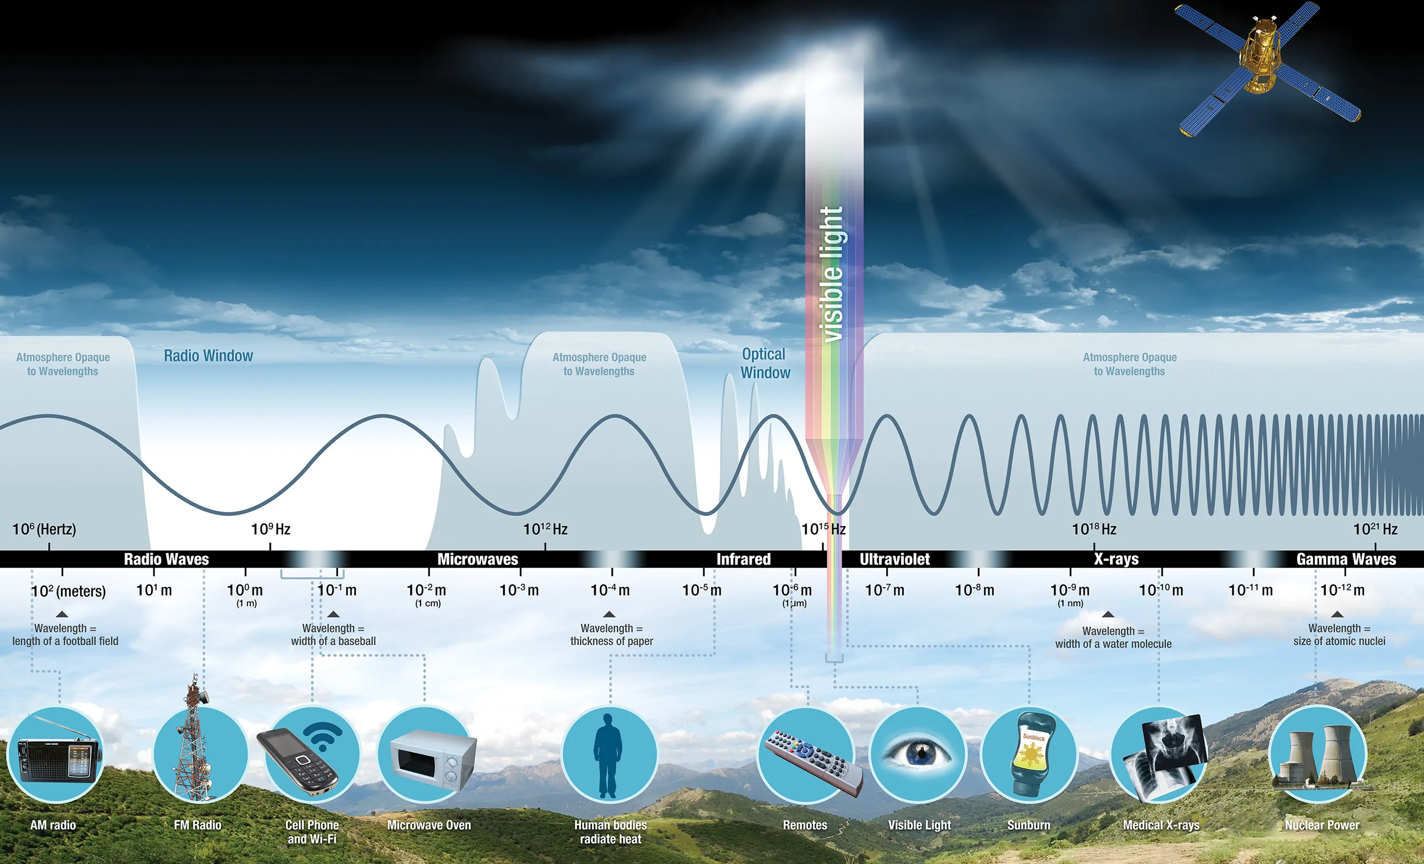
\includegraphics[scale=0.35]{./Figures/EMN} \vspace{-0.2cm}
        %\caption*{Source: National Aeronautics and Space Administration, Science Mission Directorate. (2010).}
        %%\label{fig:voltage}
    %\end{figure}
%\end{frame} 
				\begin{frame} \frametitle{\large{The Electromagnetic Spectrum}}%\vspace{-0.3cm}	
\begin{figure}[H] 
         \centering
         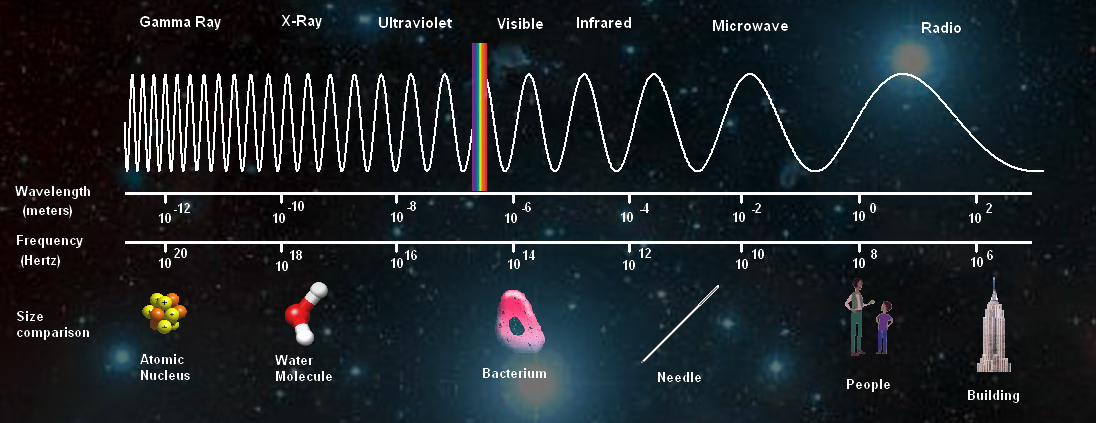
\includegraphics[scale=0.5]{./Figures/EMB} \vspace{-0.2cm}
        \caption*{\tiny{Source: Science Notes and Projects.}}
        %\label{fig:voltage}
    \end{figure}
\end{frame}

				\begin{frame} \frametitle{\large{The Electromagnetic Spectrum}}%\vspace{-0.3cm}	
\begin{figure}[H] 
         \centering
         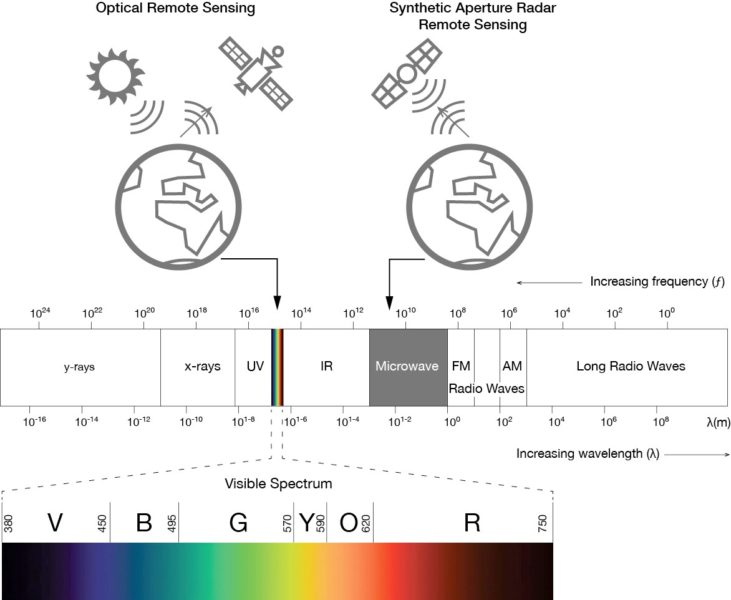
\includegraphics[scale=0.8]{./Figures/Image_op}% \vspace{-0.2cm}
        \caption*{\tiny{Source: National Aeronautics and Space Administration, Science Mission Directorate. (2010).}}
        %\label{fig:voltage}
    \end{figure}
\end{frame}
		
		\begin{frame} \frametitle{\large{Sentinel Satellites}}%\vspace{-0.3cm}	
\begin{figure}[H] 
         \centering
         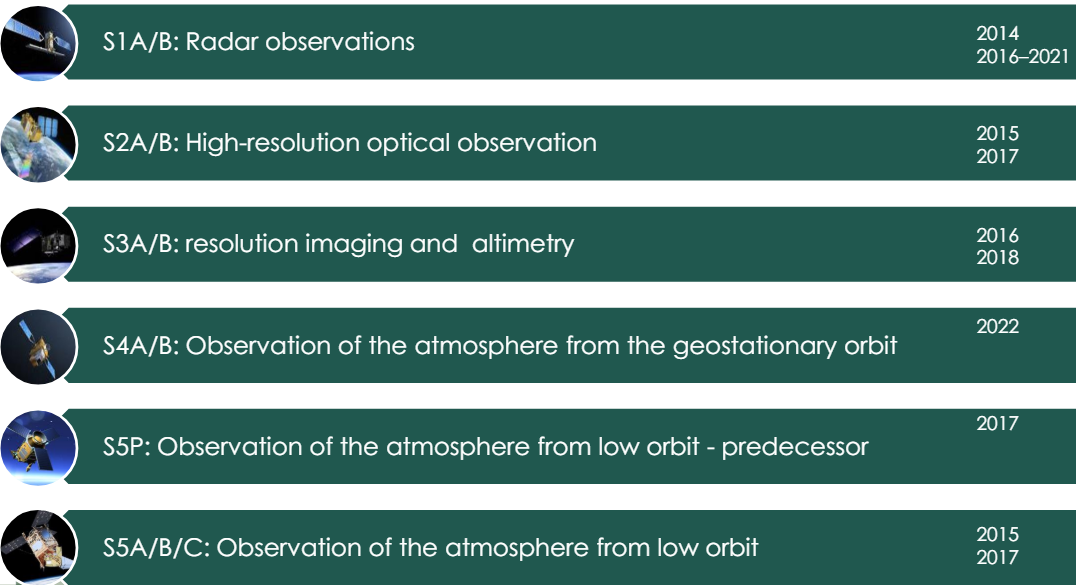
\includegraphics[scale=0.4]{./Figures/sentinel_radar} \vspace{0.1cm}
        \caption*{}
        %\label{fig:voltage}
    \end{figure}
\end{frame} 
		

\begin{frame} \frametitle{\large{The Sentinel-1 Constellation }}\vspace{-0.4cm}

 \justifying
\begin{columns}[T,onlytextwidth]
    \begin{column}{.49\textwidth}
		\animategraphics[width=8cm, height=6cm,autoplay,loop]{10}{./constelation/constelation_}{000}{241}
    \end{column}
\begin{column}{.40\textwidth}\vspace{-1.0cm}
  \begin{block}{} \vspace{-0.8cm}
		\justifying
				\end{block}%\vspace{2.8cm}				
				\begin{itemize}
				\item Radar satellite
					\item Launched by the European Space Agency (ESA)
					\item Free-and-open, globally \& regularly acquired, weather-independent Earth observation data
					\item Constellation of two C-band SAR Sensors
					\item Observation of land, forests, water, soil and agriculture
					\item Orbit repeatability 12 days, 6 days with two satellites

				\end{itemize}
    \end{column}
\end{columns}\vspace{0.2cm}
\end{frame} 

		\begin{frame} \frametitle{\large{Acquisition Concept }}%\vspace{-0.3cm}	
\begin{center}
		\animategraphics[width=12cm, height=8cm,autoplay,loop]{10}{./sentinel/sentinel_}{000}{299}
	\end{center}
\end{frame} 


		\begin{frame} \frametitle{\large{Sentinel-1 SAR data processing}}%\vspace{-0.3cm}	
\begin{figure}[H] 
         \centering
         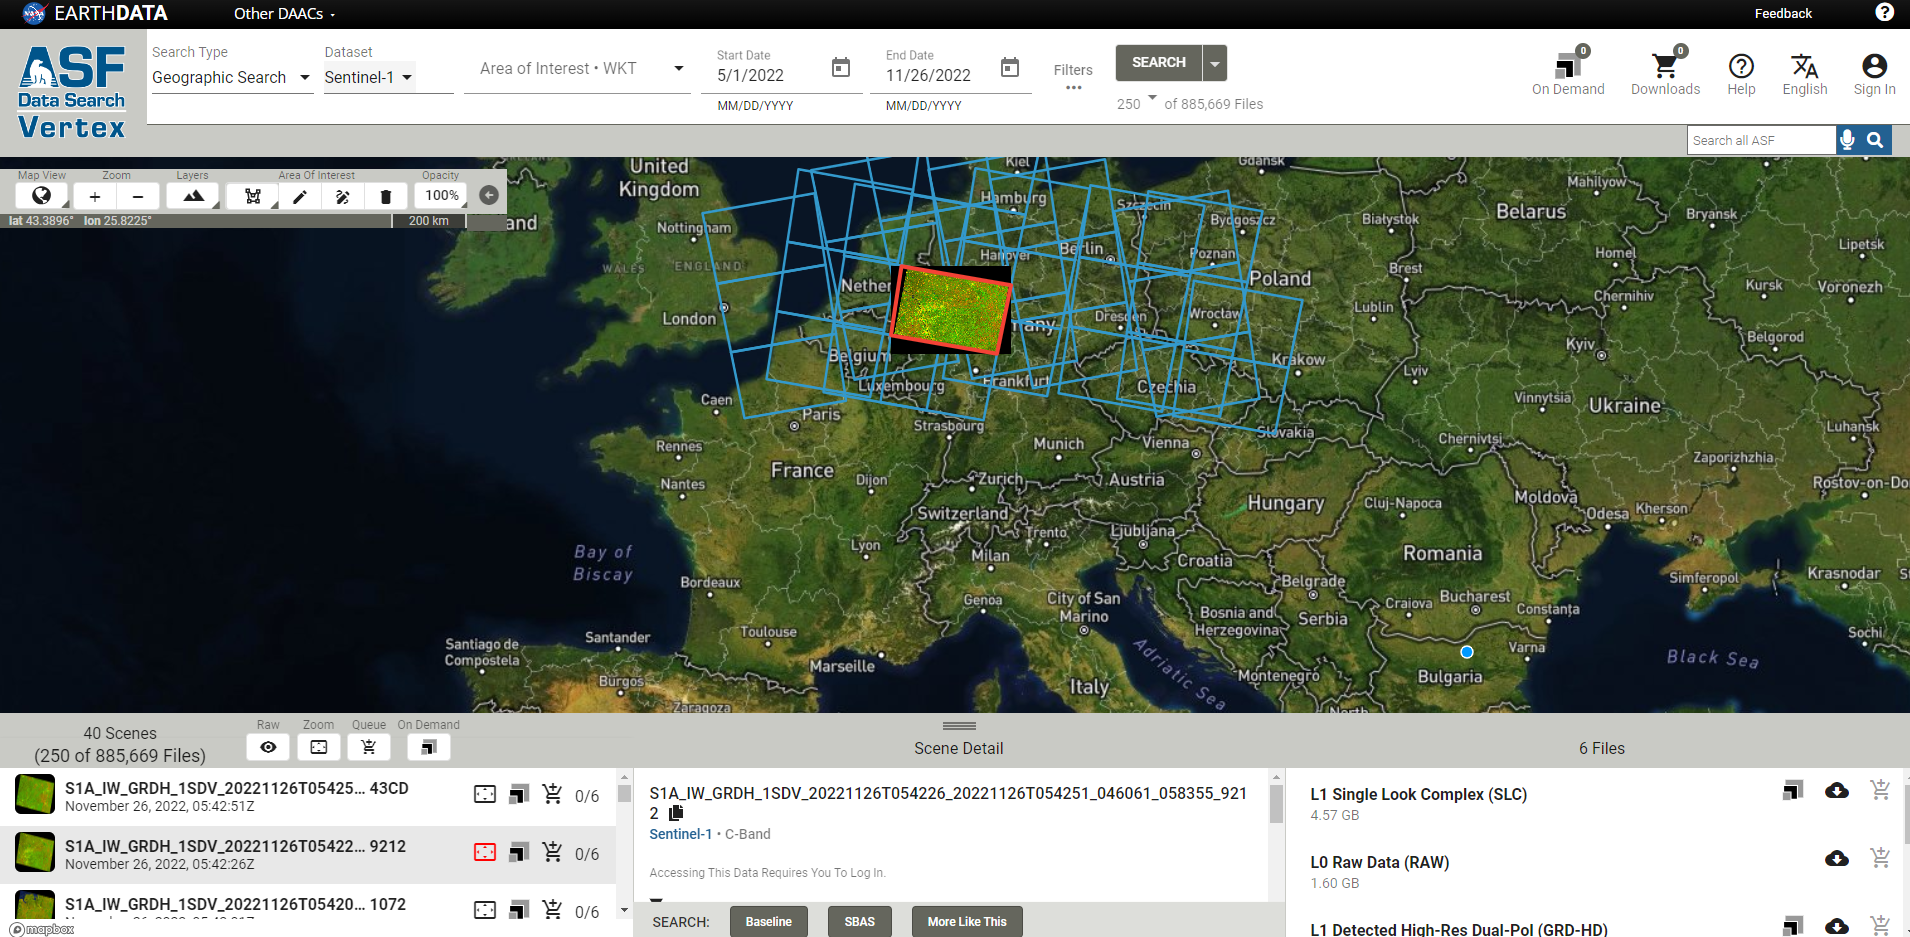
\includegraphics[scale=0.28]{./Figures/alaska1} \vspace{0.1cm}
        \caption*{}
        %\label{fig:voltage}
    \end{figure}
\end{frame} 
		
		
				\begin{frame} \frametitle{\large{Sentinel-1 SAR data processing}}%\vspace{-0.3cm}	
\begin{figure}[H] 
         \centering
         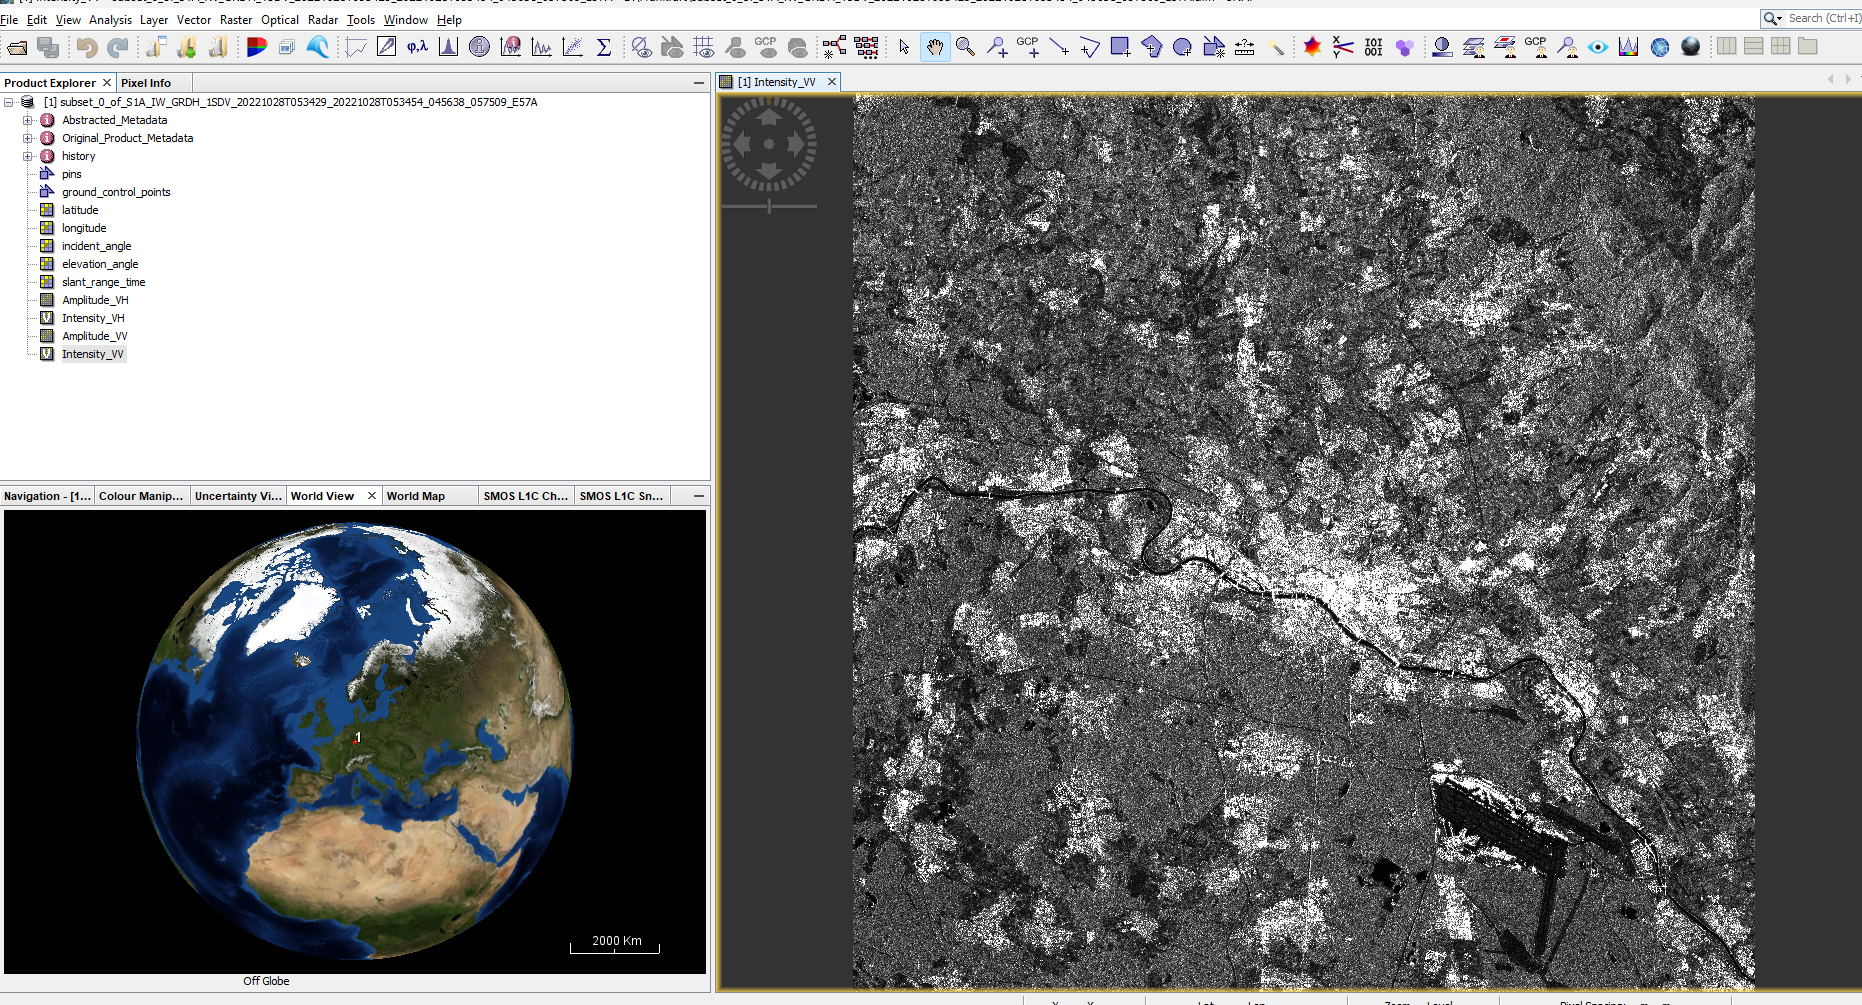
\includegraphics[scale=0.28]{./Figures/snap_1} \vspace{0.1cm}
        \caption*{}
        %\label{fig:voltage}
    \end{figure}
\end{frame} 

\section{Context and Problem Statement}
%----------------------------------------------------------------------------------------

%\begin{frame}{video}
%\centering
%\includemedia[
%label=video1,
%width=0.8\linewidth, height=0.5\linewidth,
%addresource=sentinel.mp4,
%transparent,
%activate=pageopen,
%deactivate=onclick,
%playbutton=fancy,
%flashvars={
%vid=sentinel.mp4&scaleMode=letterbox},
%]{}{VPlayer.swf}     
%\end{frame}

%\begin{frame}{animacion}
	%\begin{center}
		%\animategraphics[width=6cm, height=5cm,autoplay,loop]{10}{./sentinel/sentinel_}{000}{299}
	%\end{center}
	%\end{frame}
%
%
%\begin{frame}{animacion2}
	%\begin{center}
		%\animategraphics[width=6cm, height=5cm,autoplay,loop]{10}{./constelation/constelation_}{000}{241}
	%\end{center}
	%\end{frame}

\begin{frame} \frametitle{\large{Context}}\vspace{-0.3cm}	

 \justifying
\begin{columns}[T,onlytextwidth]
    \begin{column}{.55\textwidth}
			\begin{alertblock}{Fully Developed Speckle (FDS)}\justifying
			\vspace{0.4cm}	
Homogeneous areas in SAR images are characterized by the lack of dominant scatterers, and the surface can be considered stationary.
This is the case of the \textbf{fully developed hypothesis for the speckle}.

%The speckle noise follows a well-defined statistical distribution, typically modeled as a Gamma distribution. 
		 \vspace{0.4cm}	
	\end{alertblock}
	\begin{alertblock}{Optimal model}\justifying
	\vspace{0.2cm}	
		The \(\mathcal{G}^0\) distribution is a suitable model for SAR intensity data. %because it describes  areas with different degrees of texture. 
		It includes the \textbf{Gamma law} as a limit case that results in the presence of fully developed speckle.


	\end{alertblock}
		
    \end{column}
    \begin{column}{.40\textwidth}\vspace{-0.8cm}
		     \begin{block}{} 
		\justifying
				\begin{figure}[H]
    \centering
    \subfloat[\scriptsize{FDS (Pasture area)}]{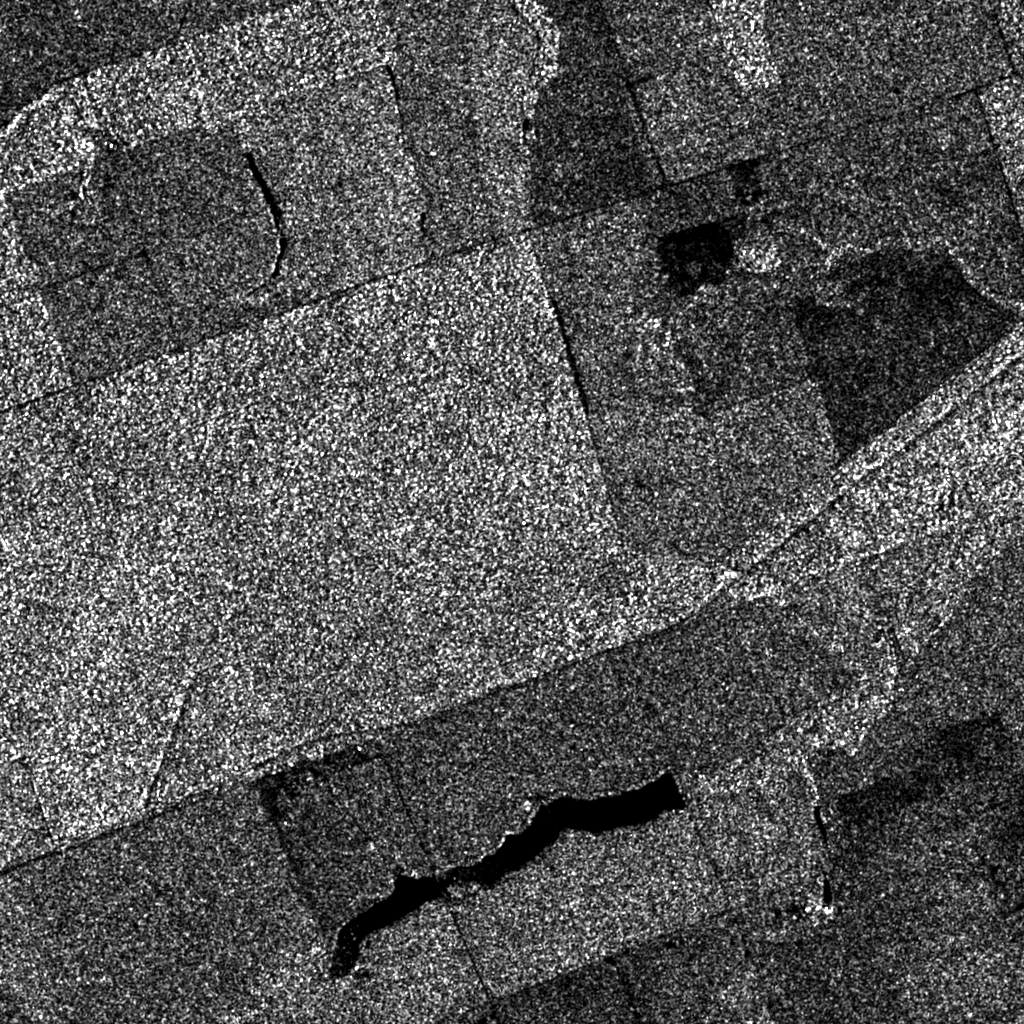
\includegraphics[width=30mm]{./Figures/Intensity_MG} }\hfill
    \subfloat[\scriptsize{Heterogeneous clutter (urban area)}]{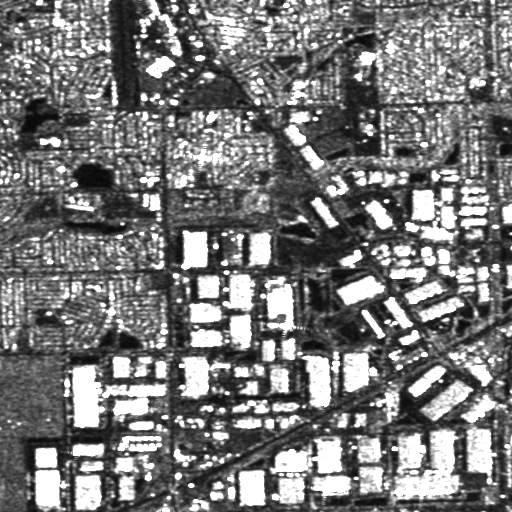
\includegraphics[width=30mm]{./Figures/urban_intensity} }\vspace{-0.4cm}
    \caption*{SAR images.}
    \label{fig:real_SAR_Images_coe}
\end{figure}
\end{block}\vspace{2.8cm}
    \end{column}
\end{columns}\vspace{0.2cm}
%\metroset{block=fill}
      %\begin{exampleblock}{Objetive}
       
      %\end{exampleblock}

\end{frame} 
%----------------------------------------------------------------------------------------
\begin{frame} \frametitle{\large{Problem and Proposal}}\vspace{0.4cm}	

 \justifying
\begin{columns}[T,onlytextwidth]
    \begin{column}{.8\textwidth}
			\begin{exampleblock}{}\justifying
Selecting the optimal statistical model to characterize speckle in SAR data presents challenges. 
\pause
\begin{itemize}
    \item Opting for the \textbf{Gamma law }with $\mathcal{G}^0$ data:
    \begin{itemize}
        \item Loss of the information about the number of scatterers.
    \end{itemize}
		\pause
    \item \textbf{Applying $\mathcal{G}^0$} under fully developed speckle:
    \begin{itemize}
        \item Tricky maximum likelihood estimation:
       Increased bias, flat likelihood, and numerical optimization may not
converge.
        
    \end{itemize}
\end{itemize}
		 
	\end{exampleblock}
	\pause
	\begin{exampleblock}{Our approach}\vspace{0.2cm}	
	\justifying
		\textcolor[rgb]{0,0,0.55}{ We propose a test statistic to distinguish between fully developed speckle and heterogeneous clutter, based on the non-parametric entropy estimation}.


	\end{exampleblock}
		
    \end{column}
    
\end{columns}\vspace{0.2cm}


\end{frame} 
%----------------------------------------------------------------------------------------
\section{Model Setup}
\begin{frame} \frametitle{\large{Model Setup}}\vspace{0.4cm}	

 \justifying
%The primary models used for intensity SAR data include the Gamma and \(\mathcal{G}_I^0\) distribution.
\begin{columns}[T,onlytextwidth]
    \begin{column}{.99\textwidth}
			\begin{exampleblock}{Intensity SAR Data}\vspace{0.4cm}	
			\justifying
We denote
\(Z \sim \Gamma_{\text{SAR}}(L, \mu)\) and
\(Z \sim \mathcal{G}_I^0(\alpha, \gamma, L)\) to indicate that \(Z\)
follows the distributions characterized by the respective probability
density functions:
\begin{align}%\large
 \textcolor[rgb]{0,0,1}{f_Z(z;L, \mu)=\frac{L^L}{\Gamma(L)\mu^L}z^{L-1}\exp\left\{-Lz/\mu\right\} \mathbbm 1_{\mathbbm R_+}(z), \label{E:gamma1}}\\ \nonumber\\
\textcolor[rgb]{0,0,1}{f_Z(z; \alpha, \gamma, L)=\frac{L^L\Gamma(L-\alpha)}{\gamma^{\alpha}\Gamma(-\alpha)\Gamma(L)}\cdot\frac{z^{L-1}}{(\gamma+Lz)^{L-\alpha}} \mathbbm 1_{\mathbbm R_+}(z),\label{E:gi01}}    
\end{align}
where \(L \geq 1\) is the number of looks, \(\Gamma(\cdot)\)
is the gamma function, and \(\mathbbm 1_{A}(z)\) is the indicator
function of the set \(A\). 
In~\eqref{E:gamma1}, \(\mu > 0\) is the mean;
in~\eqref{E:gi01} \(\gamma > 0\) is the scale, \(\alpha < -1\) measures
the roughness.
	\end{exampleblock}
	\
		
    \end{column}
    
\end{columns}\vspace{0.2cm}


\end{frame} 

%----------------------------------------------------------------------------------------
\begin{frame} \frametitle{\large{Model Setup}}\vspace{0.4cm}	

 \justifying
\begin{columns}[T,onlytextwidth]
    \begin{column}{.99\textwidth}
			\begin{block}{New Parametrization of \(\mathcal{G}_I^0\) }\justifying
			\vspace{0.4cm}
We can parametrize~\eqref{E:gi01} by the mean value: \begin{align*}
    \mu=-\frac{\gamma}{\alpha+1}.
\end{align*} 
\pause
Thus, the probability density function that characterize
the \(G_I^0(\mu, \alpha, L)\) law is \begin{align*}
       \alert<+>{f_Z(z; \mu, \alpha, L)=\frac{L^L\Gamma(L-\alpha)}{\big(-\mu(\alpha+1)\big)^{\alpha}\Gamma(-\alpha)\Gamma(L)}\cdot\frac{z^{L-1}}{\big(-\mu(\alpha+1)+Lz\big)^{L-\alpha}}\mathbb{1}_{\mathbbm R_+}(z)}.
\end{align*}
	\end{block}
	\
		
    \end{column}
    
\end{columns}%\vspace{0.2cm}
\end{frame} 

\section{Non-parametric Entropy Estimation Approach}
%----------------------------------------------------------------------------------------
\begin{frame} \frametitle{\large{Non-parametric Entropy Estimation Approach}}\vspace{0.4cm}	

 \justifying
\begin{columns}[T,onlytextwidth]
    \begin{column}{.45\textwidth}
			\begin{block}{Shannon Entropy}\justifying
 
\begin{small}
\begin{align*}
%\label{E:E-gamma}
 \textcolor[rgb]{0,0,1}{H_{\Gamma_{\text{SAR}}}(L, \mu)} \ &\textcolor[rgb]{0,0,1}{  =  L -\ln L+\ln\Gamma(L)}\\
& \textcolor[rgb]{0,0,1}{\quad +(1-L)\psi^{(0)}(L) + \ln \mu, }
\end{align*} 
\begin{align*}
%\label{E:E-GIO}
H_{G_I^0}(\mu, \alpha, L) \ &=\textcolor[rgb]{0,0,1}{ H_{\Gamma_{\text{SAR}}}} -\ln\Gamma(L-\alpha)\\
&\quad + (L-\alpha) \psi^{(0)}(L-\alpha)\\
&\quad -(1-\alpha)\psi^{(0)}(-\alpha)+\ln (-1-\alpha)\\
&\quad+\ln\Gamma(-\alpha)-L,
\end{align*}
\end{small}
where \(\psi^{(0)}(\cdot)\) is the digamma function.
		\end{block}
    \end{column}
		
    
\begin{column}{.48\textwidth}\vspace{-0.5cm}
		     \begin{block}{} 
		\justifying
				\begin{figure}[H] 
         \centering
         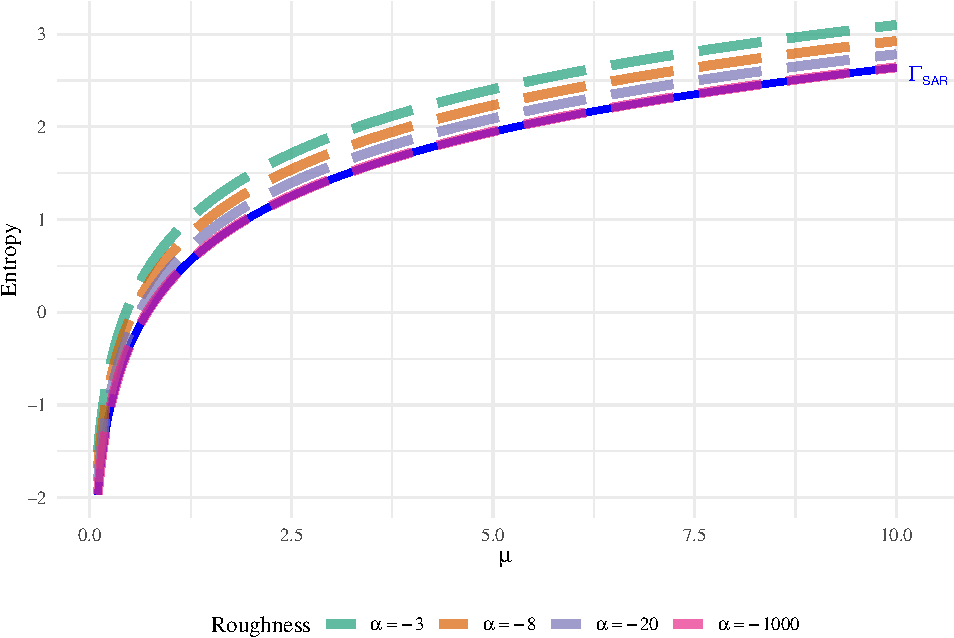
\includegraphics[scale=0.45]{./Figures/Plot_GI0_to_gamma1-1} 
        \caption*{$H_{ G_I^0}$ converges to the $H_{\Gamma_{\text{SAR}}}$, $L=8$.}
        %\label{fig:voltage}
    \end{figure}
		%\begin{block}{} 
		%\justifying
%\end{block}
\end{block}\vspace{2.8cm}
    \end{column}
\end{columns}\vspace{0.2cm}
%\metroset{block=fill}
      %\begin{exampleblock}{Objetive}
       
      %\end{exampleblock}

\end{frame} 


%----------------------------------------------------------------------------------------
\begin{frame} \frametitle{\large{Non-parametric Entropy Estimation Approach}}\vspace{0.4cm}	

 \justifying
\begin{figure}[htb]
  \centering
  \begin{subfigure}[b]{0.3\textwidth}
    \centering
    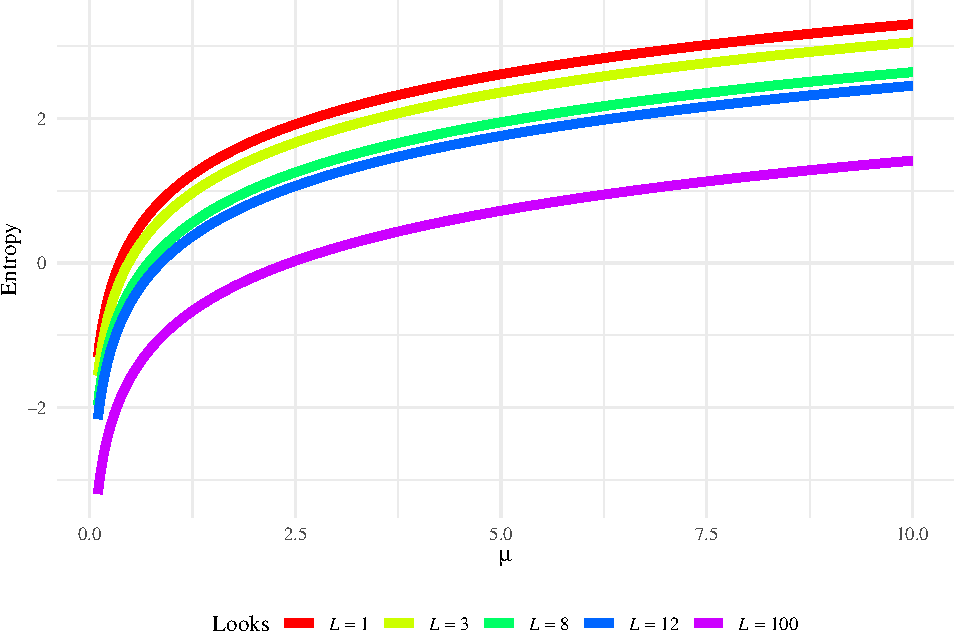
\includegraphics[width=1.5\textwidth]{../../Figures/PDF/PlotGammaSAR-1}
    \caption{The Shannon Entropy of $\Gamma_{\text{SAR}}$.}
    \label{fig:H1}
  \end{subfigure}
  \hfill
  \begin{subfigure}[b]{0.5\textwidth}
    \centering
    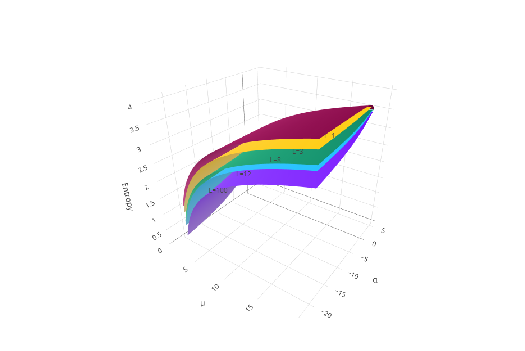
\includegraphics[width=9cm, height=5cm]{../../Figures/PDF/3d_lab}
    \caption{The Shannon Entropy of $G_I^0$.}
    \label{fig:H2}
  \end{subfigure}
  \caption{Theoretical entropies for $\Gamma_{\text{SAR}}$ and $G_I^0$ distributions.}
  \label{fig:all_H}
\end{figure}

\end{frame} 
%----------------------------------------------------------------------------------------


\begin{frame} \frametitle{\large{Non-parametric Entropy Estimation Approach}}

 \justifying
\begin{columns}[T,onlytextwidth]
    \begin{column}{.45\textwidth}
			\begin{block}{}\justifying
 %Non-parametric approaches do not use $\widehat{\bm{\theta}}$ as a proxy. Instead, they rely on differences between order statistics.

Vasicek introduced an  non-parametric estimator in 1976: \begin{equation*}
\label{E:Vas}
    \alert<+>{\widehat{H}_{\text{V}}(\bm{Z})=\frac{1}{n}\sum_{i=1}^{n}\ln\left[\frac{n}{2m}\left(Z_{(i+m)}-Z_{(i-m)}\right)\right],}
    \end{equation*} where
\(Z_{(i+m)}-Z_{(i-m)}\) is the \(m\)-spacing and
\(Z_{(1)}\leq Z_{(2)}\leq\ldots\leq Z_{(n)}\) are the \textbf{order statistics.}

\pause

We consider superior adaptations:
\begin{itemize}
\item $\left[\text{Ebrahimi et al., 1994}\right]$: \(\widehat{H}_{\mathrm{E}}\).
\item  $\left[\text{Correa, 1995}\right]$: \(\widehat{H}_{\text{C}}\).
\item  $\left[\text{Al Omary, 2014}\right]$: \(\widehat{H}_{\mathrm{AO}}\).
\end{itemize}
		\end{block}
    \end{column}
		
  \pause  
\begin{column}{.48\textwidth}\vspace{-0.1cm}
%\metroset{block=fill}
\begin{exampleblock}{Enhanced Bootstrap Technique}
        \begin{align*}
\textcolor[rgb]{0,0,1}{\widetilde{H} = 2\widehat{\theta}(\bm{Z}) - \frac{1}{B}\sum_{b=1}^B \widehat{\theta}_b(\bm{Z}^{(b)})}
\end{align*} 
      \end{exampleblock}
					     \begin{block}{} \vspace{-0.8cm}
		\justifying
				\begin{figure}[H]
{\centering 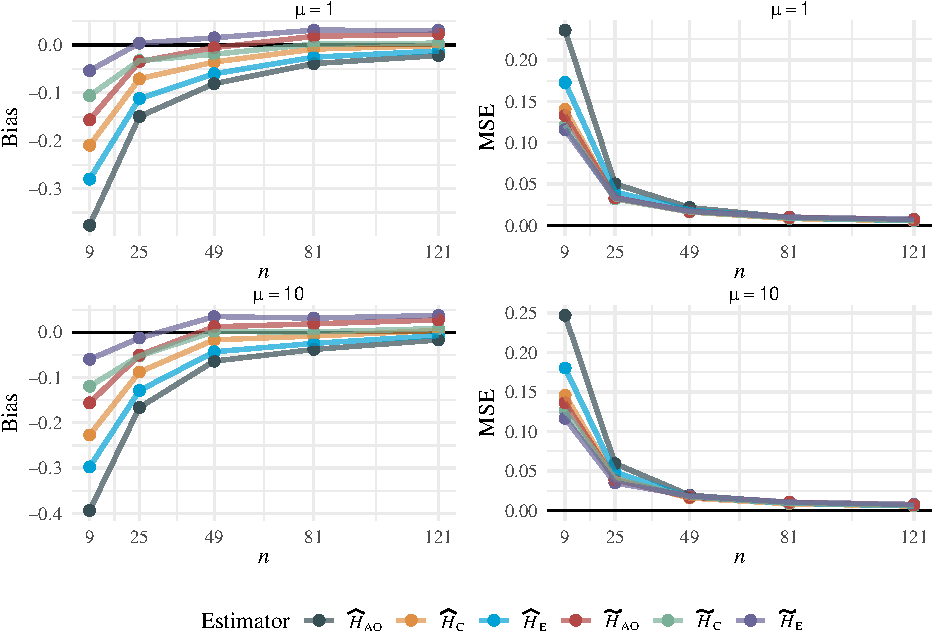
\includegraphics[width=1.0\linewidth]{../../Figures/PDF/Plot_bias_mse_gi0-2} 

}
\caption{Bias and MSE of the entropy estimators for the $\Gamma_{\text{SAR}}$, with $L=5$.}\label{fig:Plot_bias_mse_gi0}
\end{figure}


		%\begin{block}{} 
		%\justifying
%\end{block}
\end{block}\vspace{2.8cm}
    \end{column}
\end{columns}\vspace{0.2cm}
%\metroset{block=fill}
      %\begin{exampleblock}{Objetive}
       
      %\end{exampleblock}

\end{frame} 

%----------------------------------------------------------------------------------------

\begin{frame} \frametitle{\large{Non-parametric Entropy Estimation Approach}}

\begin{table}[htb]
\centering
\caption{Test accuracy and processing time for each bootstrap-improved estimator. }
\resizebox{0.6\textwidth}{!}{
\small
\begin{tabu} to \linewidth {>{\centering}X>{\centering}X>{\centering}X>{\centering}X>{\centering}X}
\toprule
\textbf{Estimator} & $\bm{L}$ & $\bm{n}$ & $S(\bm{Z}; L)$ & \textbf{Time (s)}\\
\midrule
 &  & $25$ & $-0.00152$ & 22.53\\

 &  & $49$ & $\phantom{-}0.00515$ & 40.35\\

 &  & $81$ & $\phantom{-}0.00625$ & 63.93\\

 & \multirow{-4}{*}[1.5\dimexpr\aboverulesep+\belowrulesep+\cmidrulewidth]{\centering\arraybackslash $2$} & $121$ & $\phantom{-}0.00751$ & 97.06\\

\cline{3-5}
 &  & $25$ & $-0.04332$ & 22.25\\

 &  & $49$ & $-0.01659$ & 33.42\\

 &  & $81$ & $-0.00393$ & 50.94\\

\multirow{-8}{*}[3.5\dimexpr\aboverulesep+\belowrulesep+\cmidrulewidth]{\centering\arraybackslash $\widetilde{H}_{\text{C}}$} & \multirow{-4}{*}[1.5\dimexpr\aboverulesep+\belowrulesep+\cmidrulewidth]{\centering\arraybackslash $8$} & $121$ & $\phantom{-}0.00261$ & 97.35\\
\cmidrule{1-5}
 &  & $25$ & $\phantom{-}0.02204$ & 4.66\\

 &  & $49$ & $\phantom{-}0.03452$ & 5.55\\

 &  & $81$ & $\phantom{-}0.03195$ & 6.89\\

 & \multirow{-4}{*}[1.5\dimexpr\aboverulesep+\belowrulesep+\cmidrulewidth]{\centering\arraybackslash $2$} & $121$ & $\phantom{-}0.03012$ & 7.90\\

\cline{3-5}
 &  & $25$ & $\phantom{-}0.00801$ & 4.81\\

 &  & $49$ & $\phantom{-}0.01654$ & 5.43\\

 &  & $81$ & $\phantom{-}0.03036$ & 6.38\\

\multirow{-8}{*}[3.5\dimexpr\aboverulesep+\belowrulesep+\cmidrulewidth]{\centering\arraybackslash $\widetilde{H}_{\text{E}}$} & \multirow{-4}{*}[1.5\dimexpr\aboverulesep+\belowrulesep+\cmidrulewidth]{\centering\arraybackslash $8$} & $121$ & $\phantom{-}0.03137$ & 7.46\\
\cmidrule{1-5}
 &  & $25$ & $-0.01935$ & 4.61\\

 &  & $49$ & $\phantom{-}0.00786$ & 5.19\\

 &  & $81$ & $\phantom{-}0.01995$ & 6.70\\

 & \multirow{-4}{*}[1.5\dimexpr\aboverulesep+\belowrulesep+\cmidrulewidth]{\centering\arraybackslash $2$} & $121$ & $\phantom{-}0.01741$ & 7.41\\

\cline{3-5}
 &  & $25$ & $-0.04020$ & 4.74\\

 &  & $49$ & $\phantom{-}0.00047$ & 5.35\\

 &  & $81$ & $\phantom{-}0.01176$ & 6.21\\

\multirow{-8}{*}[3.5\dimexpr\aboverulesep+\belowrulesep+\cmidrulewidth]{\centering\arraybackslash $\widetilde{H}_{\text{AO}}$} & \multirow{-4}{*}[1.5\dimexpr\aboverulesep+\belowrulesep+\cmidrulewidth]{\centering\arraybackslash $8$} & $121$ & $\phantom{-}0.02019$ & 7.48\\
\bottomrule
\end{tabu}}
\end{table}



\end{frame} 


\section{Hypothesis Testing}
\begin{frame} \frametitle{\large{Hypothesis Testing }}\vspace{0.1cm}

 \justifying
\begin{columns}[T,onlytextwidth]
    \begin{column}{.45\textwidth}
			\begin{block}{}\justifying
 We aim at testing the following hypotheses:

\[\textcolor[rgb]{0,0,1}{
 \begin{cases}\mathcal{H}_0: \widetilde{H}^*= H_{\Gamma_{\text{SAR}}}\\ 
  \mathcal{H}_1:\widetilde{H}^*= H_{G_I^0}.\end{cases}}
\] In other words, we verify the hypothesis that the data are
fully-developed speckle with the following \textbf{test statistic}:
\pause
\begin{equation*}
%\label{Eq:test_e}
\alert<+>{S(\bm{Z};L)= \widetilde{H}-\left[H_{\Gamma_{\text{SAR}}}(L)+\ln \widebar{\bm{Z}}\right].}
\end{equation*} The values should be around zero under the null
hypothesis and far otherwise.
		\end{block}
    \end{column}
		
\pause
\begin{column}{.52\textwidth}\vspace{-1.0cm}
  \begin{block}{} %\vspace{-0.8cm}
		\justifying
				\begin{figure}[H] 
         \centering
         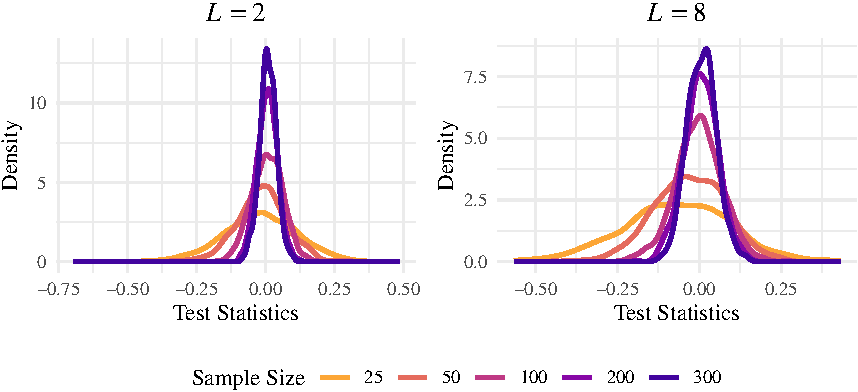
\includegraphics[scale=0.4]{./Figures/Plot_density-1} \vspace{-0.4cm}
        \caption*{\tiny{Empirical density  under the null hypothesis.}}
        %\label{fig:voltage}
    \end{figure}
\pause
\vspace{-1.0cm}
\setlength{\tabcolsep}{10pt}
\begin{table}
\colorbox{violet!10}{%
 	\resizebox{0.8\textwidth}{!}{%
  \renewcommand{\arraystretch}{1.3}
	\begin{tabular}[t]{lrrrrrrrl}
\toprule
\multicolumn{1}{c}{$\bm L$} & \multicolumn{1}{c}{$\bm n$} & \multicolumn{1}{c}{\textbf{Mean}} & \multicolumn{1}{c}{\textbf{SD}} & \multicolumn{1}{c}{\textbf{Var}}  & \multicolumn{1}{c}{\textbf{SK}} & \multicolumn{1}{c}{\textbf{EK}} & \multicolumn{1}{c}{$p$-\textbf{value}}\\
\midrule
 & $25$ & $-0.0199$ & $\phantom{-}0.1370$ & $\phantom{-}0.0188$  & $-0.3492$ & $\phantom{-}1.2320$ & $\phantom{-}0.0586$\\

 & $50$ & $-0.0145$ & $\phantom{-}0.0896$ & $\phantom{-}0.0080$  & $-0.1367$ & $\phantom{-}0.4826$ & $\phantom{-}0.0418$\\

 & $100$ & $\phantom{-}0.0064$ & $\phantom{-}0.0562$ & $\phantom{-}0.0032$  & $-0.0623$ & $-0.1617$ & $\phantom{-}0.3938$\\

 & $200$ & $\phantom{-}0.0067$ & $\phantom{-}0.0361$ & $\phantom{-}0.0013$  & $\phantom{-}0.0199$ & $-0.0305$ & $\phantom{-}0.9273$\\

\multirow{-5}{*}[2\dimexpr\aboverulesep+\belowrulesep+\cmidrulewidth]{\raggedright\arraybackslash 2} & $300$ & $\phantom{-}0.0093$ & $\phantom{-}0.0309$ & $\phantom{-}0.0010$  & $\phantom{-}0.0119$ & $\phantom{-}0.3522$ & $\phantom{-}0.1293$\\
\cmidrule{1-8}
 & $25$ & $-0.0696$ & $\phantom{-}0.1623$ & $\phantom{-}0.0264$  & $-0.1096$ & $\phantom{-}0.0158$ & $\phantom{-}0.1658$\\

 & $50$ & $-0.0301$ & $\phantom{-}0.1082$ & $\phantom{-}0.0117$  & $-0.1741$ & $\phantom{-}0.0531$ & $\phantom{-}0.2961$\\

 & $100$ & $-0.0025$ & $\phantom{-}0.0711$ & $\phantom{-}0.0051$  & $-0.0408$ & $\phantom{-}0.3446$ & $\phantom{-}0.2279$\\

 & $200$ & $\phantom{-}0.0046$ & $\phantom{-}0.0520$ & $\phantom{-}0.0027$  & $-0.0873$ & $\phantom{-}0.0466$ & $\phantom{-}0.5663$\\

\multirow{-5}{*}[2\dimexpr\aboverulesep+\belowrulesep+\cmidrulewidth]{\raggedright\arraybackslash 8} & $300$ & $\phantom{-}0.0070$ & $\phantom{-}0.0448$ & $\phantom{-}0.0020$  & $\phantom{-}0.0818$ & $\phantom{-}0.0306$ & $\phantom{-}0.5431$\\
\bottomrule
\end{tabular}}}
\caption*{\label{tab:table_stat_combined}\tiny{Descriptive analysis of $S(\bm Z; L)$ to verify the normality of the data with $L\in\left\{2, 8\right\}$ and $\mu=1$.}}
\end{table}


\end{block}\vspace{2.8cm}
    \end{column}
\end{columns}\vspace{0.2cm}
%\metroset{block=fill}
      %\begin{exampleblock}{Objetive}
       
      %\end{exampleblock}

\end{frame} 


\begin{frame} \frametitle{\large{Hypothesis Testing }}\vspace{0.5cm}

 \justifying
\begin{columns}[T,onlytextwidth]
    \begin{column}{.45\textwidth}
			\begin{block}{\small{\quad  \quad Empirical densities}}\justifying
				\begin{figure}[H] 
         \centering
         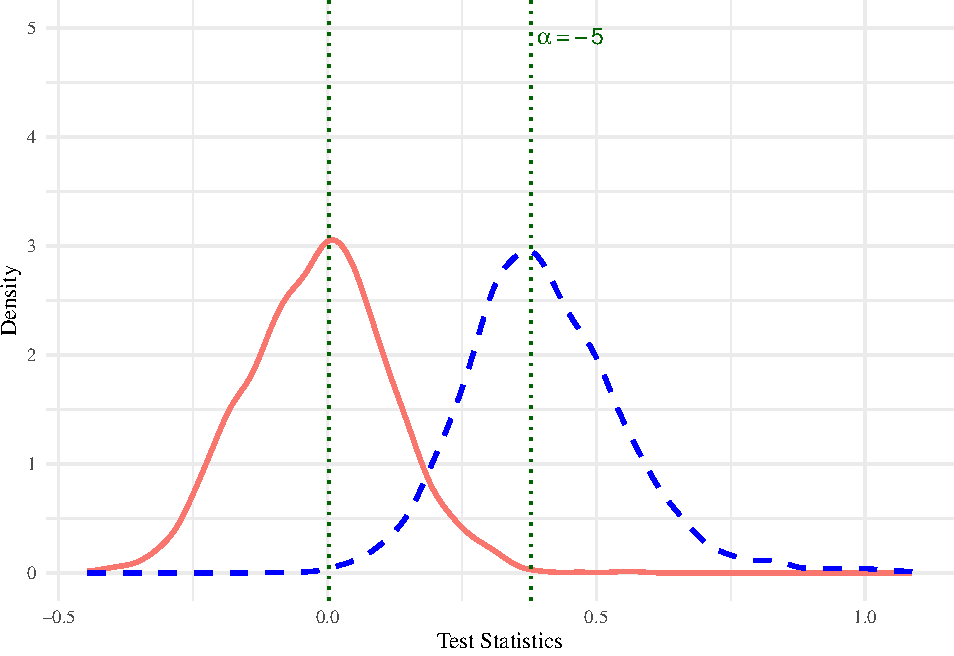
\includegraphics[scale=0.4]{./Figures/Plot_empirical_test-1} \vspace{-0.4cm}
        \caption*{\tiny{Empirical distributions under the null (centered around zero) and alternative hypotheses (e.g., $\alpha=-5$, showing a shift from zero), with $\mu=1$ and $L=8$.}}
        %\label{fig:voltage}
    \end{figure}
		\end{block}
    \end{column}
\begin{column}{.52\textwidth}%\vspace{-1.0cm}
  \begin{block}{\small{\quad \quad Size and Power of the proposed test.}} %\vspace{-0.8cm}
		\justifying
				
		%\begin{block}{} 
		%\justifying
%\end{block}
%\vspace{-1.0cm}
\setlength{\tabcolsep}{10pt}
\begin{table}
\colorbox{violet!10}{%
 	\resizebox{0.9\textwidth}{!}{%
  \renewcommand{\arraystretch}{1.3}
	\begin{tabular}[t]{lccccccc}
\toprule
\multicolumn{1}{c}{ } & \multicolumn{1}{c}{ } & \multicolumn{3}{c}{\textbf{Size}} & \multicolumn{3}{c}{\textbf{Power}} \\
\cmidrule(l{3pt}r{3pt}){3-5} \cmidrule(l{3pt}r{3pt}){6-8}
\multicolumn{1}{c}{$\bm L$} & \multicolumn{1}{c}{$\bm n$} & \multicolumn{1}{c}{$1\%$} & \multicolumn{1}{c}{$5\%$} & \multicolumn{1}{c}{$10\%$} & \multicolumn{1}{c}{$1\%$} & \multicolumn{1}{c}{$5\%$} & \multicolumn{1}{c}{$10\%$}\\
\midrule
 & 25 & $\phantom{-}0.016$ & $\phantom{-}0.071$ & $\phantom{-}0.117$ & $\phantom{-}0.564$ & $\phantom{-}0.672$ & $\phantom{-}0.745$\\

 & 50 & $\phantom{-}0.014$ & $\phantom{-}0.052$ & $\phantom{-}0.113$ & $\phantom{-}0.640$ & $\phantom{-}0.754$ & $\phantom{-}0.806$\\

 & 100 & $\phantom{-}0.010$ & $\phantom{-}0.057$ & $\phantom{-}0.103$ & $\phantom{-}0.738$ & $\phantom{-}0.838$ & $\phantom{-}0.885$\\

 & 200 & $\phantom{-}0.010$ & $\phantom{-}0.054$ & $\phantom{-}0.092$ & $\phantom{-}0.807$ & $\phantom{-}0.937$ & $\phantom{-}0.963$\\

\multirow{-5}{*}[2\dimexpr\aboverulesep+\belowrulesep+\cmidrulewidth]{\raggedright\arraybackslash 5} & 300 & $\phantom{-}0.007$ & $\phantom{-}0.058$ & $\phantom{-}0.107$ & $\phantom{-}0.850$ & $\phantom{-}0.961$ & $\phantom{-}0.988$\\
\cmidrule{1-8}
 & 25 & $\phantom{-}0.024$ & $\phantom{-}0.076$ & $\phantom{-}0.129$ & $\phantom{-}0.747$ & $\phantom{-}0.844$ & $\phantom{-}0.838$\\

 & 50 & $\phantom{-}0.015$ & $\phantom{-}0.055$ & $\phantom{-}0.104$ & $\phantom{-}0.857$ & $\phantom{-}0.919$ & $\phantom{-}0.939$\\

 & 100 & $\phantom{-}0.006$ & $\phantom{-}0.052$ & $\phantom{-}0.099$ & $\phantom{-}0.958$ & $\phantom{-}0.984$ & $\phantom{-}0.985$\\

 & 200 & $\phantom{-}0.014$ & $\phantom{-}0.043$ & $\phantom{-}0.109$ & $\phantom{-}0.989$ & $\phantom{-}0.999$ & $\phantom{-}1.000$\\

\multirow{-5}{*}[2\dimexpr\aboverulesep+\belowrulesep+\cmidrulewidth]{\raggedright\arraybackslash 8} & 300 & $\phantom{-}0.014$ & $\phantom{-}0.041$ & $\phantom{-}0.106$ & $\phantom{-}1.000$ & $\phantom{-}1.000$ & $\phantom{-}1.000$\\
\bottomrule
\end{tabular}}}
%\caption{\label{}\tiny{Size and Power of the proposed test.}}
\end{table}


\end{block}\vspace{2.8cm}
    \end{column}
\end{columns}\vspace{0.2cm}
%\metroset{block=fill}
      %\begin{exampleblock}{Objetive}
       
      %\end{exampleblock}

\end{frame} 

\section{The Proposed Test Based on Coefficient of Variation and a Robust Alternative}

\begin{frame} \frametitle{{ The Proposed Test Based on Coefficient of Variation and a Robust Alternative}}\vspace{-0.1cm}

\justifying
\begin{columns}[T,onlytextwidth]
    \begin{column}{.8\textwidth}
			\begin{exampleblock}{}\justifying
In addition to the \(S_{\widetilde{H}_{\text{AO}}}(\bm{Z}; L)\) test, we
also propose a test statistic based on the classical CV. This test
statistic is defined as follows: \begin{align}
    T_{\text{CV}}=\frac{S}{\overline{Z}},
\end{align} where \(S\) and \(\overline{Z}\) are the sample standard
deviation and mean, respectively.


Similarly, we use another test statistic based on the ratio of the MnAD
to the median. This statistic is given by: \begin{align}
    T_{\text{CV}_{\text{MnAD}}}=\frac{\text{MnAD}}{\text{Median}}.
\end{align}

We proceed to identify suitable models for these estimators of the CV,
and then form test statistics.
		 
	\end{exampleblock}
	
		
    \end{column}
    
\end{columns}\vspace{0.2cm}

\end{frame} 


	\begin{frame} \frametitle{\large{Model Selection Criterion }}%\vspace{-0.3cm}	
\begin{table}[H]
\centering\centering
\caption{\label{tab:table_aic_gamma}AIC and BIC values for evaluating the best distribution with CV data from $\Gamma_{\text{SAR}}$.}
\resizebox{\ifdim\width>\linewidth\linewidth\else\width\fi}{!}{
\begin{tabu} to \linewidth {>{\centering}X>{\centering}X>{\centering}X>{\centering}X>{\raggedleft}X>{\raggedleft}X>{\raggedleft}X}
\toprule
\multicolumn{1}{c}{\textbf{Criterion}} & \multicolumn{1}{c}{$\bm{n}$} & \multicolumn{1}{c}{\textbf{Normal}} & \multicolumn{1}{c}{\textbf{Lognormal}} & \multicolumn{1}{c}{\textbf{Gamma}} & \multicolumn{1}{c}{\textbf{Weibull}} & \multicolumn{1}{c}{\textbf{Inverse Gaussian}}\\
\midrule
 & $25$ & $-38031.9$ & $-38266.7$ & $-38311.8$ & $-36413.2$ & $-38261.6$\\

 & $49$ & $-47698.2$ & $-47913.7$ & $-47905.6$ & $-45554.0$ & $-47911.6$\\

 & $81$ & $-55382.1$ & $-55494.7$ & $-55494.9$ & $-53220.4$ & $-55493.8$\\

\multirow{-4}{*}[1.5\dimexpr\aboverulesep+\belowrulesep+\cmidrulewidth]{\centering\arraybackslash AIC} & $121$ & $-61344.9$ & $-61470.8$ & $-61453.8$ & $-58876.0$ & $-61470.5$\\
\cmidrule{1-7}
 & $25$ & $-38016.7$ & $-38251.5$ & $-38296.6$ & $-36398.0$ & $-38246.4$\\

 & $49$ & $-47683.0$ & $-47898.5$ & $-47890.4$ & $-45538.7$ & $-47896.4$\\

 & $81$ & $-55366.9$ & $-55479.5$ & $-55479.6$ & $-53205.2$ & $-55478.6$\\

\multirow{-4}{*}[1.5\dimexpr\aboverulesep+\belowrulesep+\cmidrulewidth]{\centering\arraybackslash BIC} & $121$ & $-61329.7$ & $-61455.6$ & $-61438.6$ & $-58860.8$ & $-61455.2$\\
\bottomrule
\end{tabu}}
\end{table}

\end{frame} 


		\begin{frame} \frametitle{\large{Model Selection Criterion}}%\vspace{-0.3cm}	
\begin{figure}[H]

{\centering 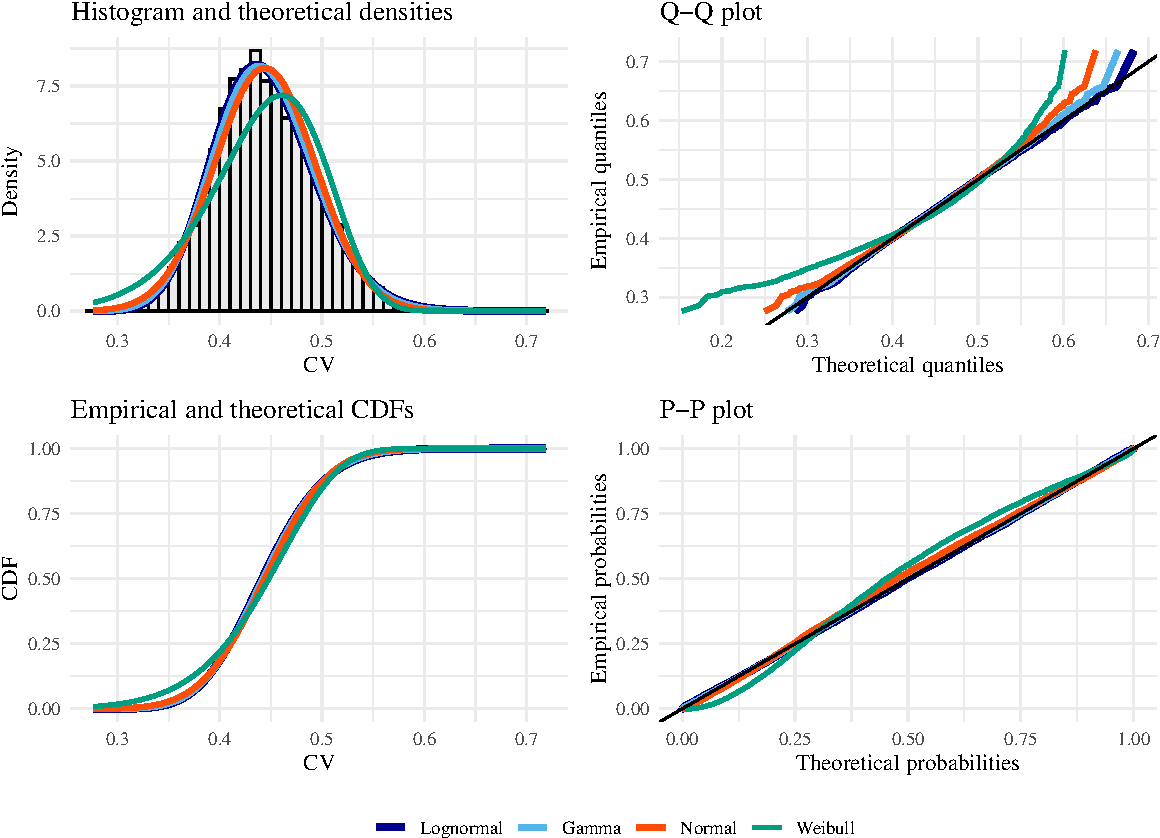
\includegraphics[width=0.8\linewidth]{../../Figures/PDF/Plot_cv_gamma-1} 

}

\caption{Goodness of fit plots for evaluating the best distribution with CV data from $\Gamma_{\text{SAR}}$ (under the null hypothesis), with $n=49$, $L=5$, and $\mu=1$.}\label{fig:Plot_cv_gamma}
\end{figure}



\end{frame} 
		
		
				%\begin{frame} \frametitle{\large{Model Selection Criterion}}%\vspace{-0.3cm}	
%{\centering 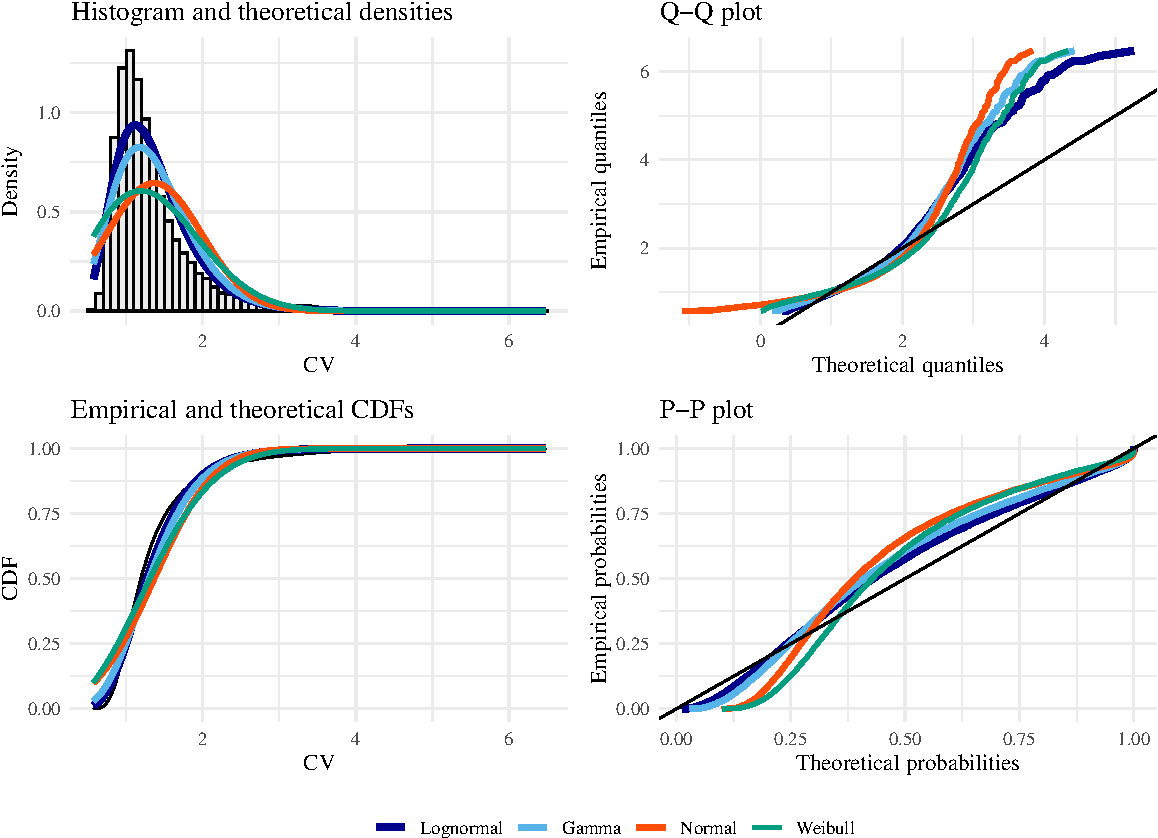
\includegraphics[width=0.8\linewidth]{../../Figures/PDF/Plot_cv-1} 
%
%}
%
%\caption{Goodness of fit plots for evaluating the best distribution with $\text{CV}$ data from $G_I^0$ (under the alternative hypothesis), with  $n=49$, $L=5$, $\mu=1$, and $\alpha=-3$.}\label{fig:Plot_cv}
%\end{figure}
%\end{frame} 


\section{Application to Simulated and SAR Data}



\begin{frame} \frametitle{\large{Simulated Data }}\vspace{-0.1cm}
%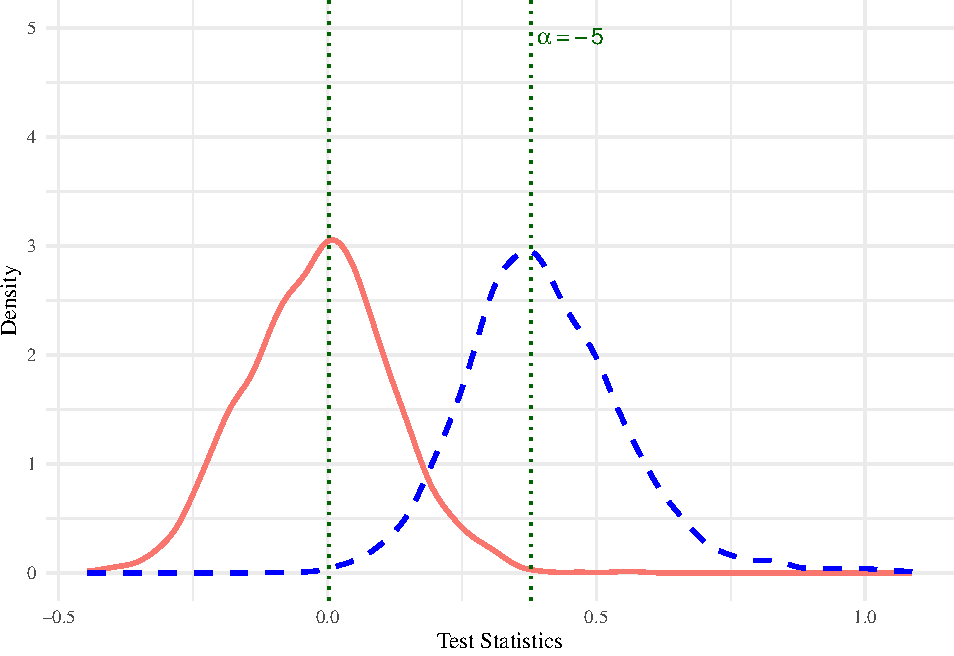
\includegraphics[scale=0.4]{./Figures/Plot_empirical_test-1} \vspace{-0.4cm}

\begin{figure}[H]
  \centering
  \begin{subfigure}[b]{0.38\textwidth}
    \centering
    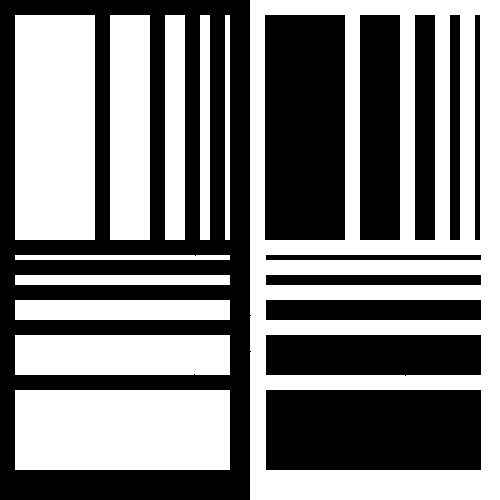
\includegraphics[width=60mm]{../../Figures/PNG/Phantom1}
    \caption{Phantom.}
    \label{fig:sim_Phantom_1}
  \end{subfigure}
  \hfill
  \begin{subfigure}[b]{0.57\textwidth}
    \centering
    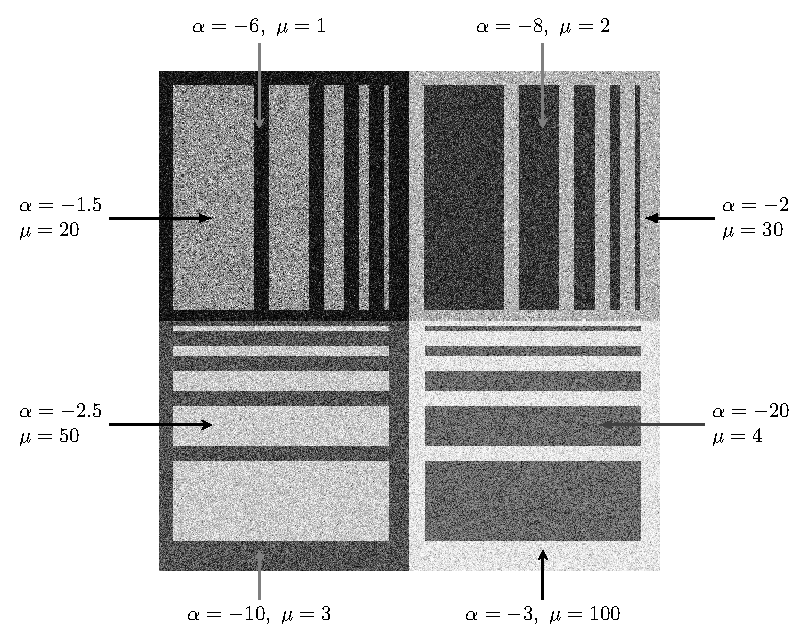
\includegraphics[width=79mm]{../../Figures/PNG/Phantom_label/Phantom_labels}
    \caption{Simulated image, varying $\alpha$ and $\mu$, with $L=5$.}
    \label{fig:sim_Phantom_2}
  \end{subfigure}
  \caption{Synthetic dataset.}
  \label{fig:sim_Phantom}
\end{figure}
 
\end{frame} 

\begin{frame} \frametitle{\large{Simulated Data }}\vspace{-0.1cm}
%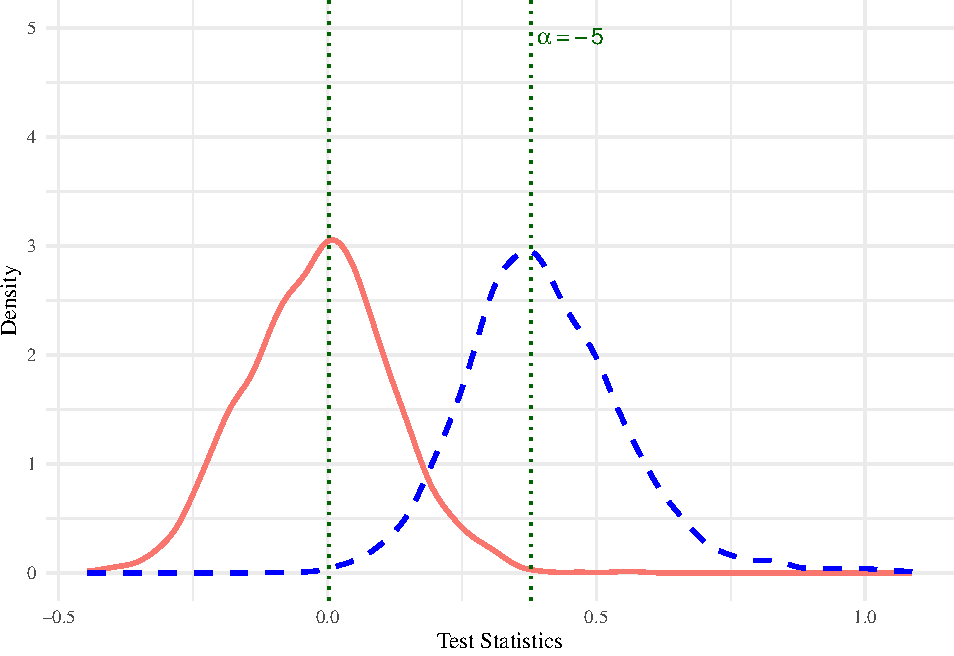
\includegraphics[scale=0.4]{./Figures/Plot_empirical_test-1} \vspace{-0.4cm}

\begin{figure}[H]
  \centering
  \begin{subfigure}[b]{0.3\textwidth}
    \centering
    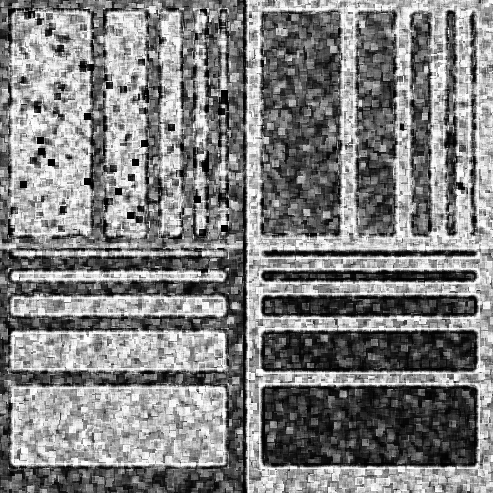
\includegraphics[width=\textwidth]{../../Figures/PNG/Entropy_Phantom_4_z1_200}
    \caption{$S_{\widetilde{H}_{\text{AO}}}(\bm{Z}; L)$}
    \label{fig:sim_results-1}
  \end{subfigure}
  \hfill
  \begin{subfigure}[b]{0.3\textwidth}
    \centering
    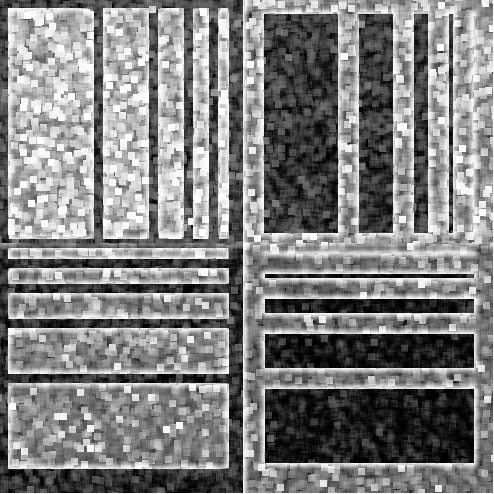
\includegraphics[width=\textwidth]{../../Figures/PNG/cv_Phantom_4_z1}
    \caption{$T_\text{CV}$}
    \label{fig:sim_results-2}
  \end{subfigure}
  \hfill
  \begin{subfigure}[b]{0.3\textwidth}
    \centering
    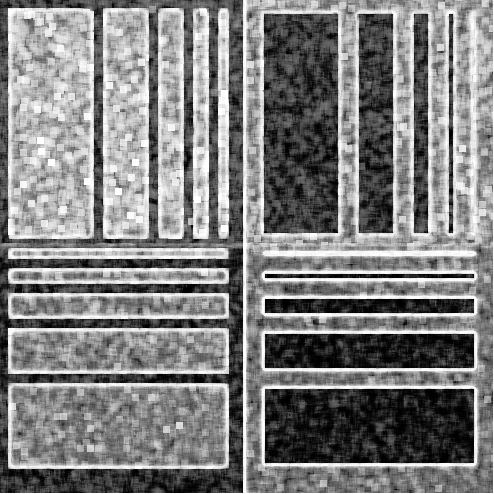
\includegraphics[width=\textwidth]{../../Figures/PNG/mnad_Phantom_z1}
    \caption{$T_{\text{CV}_{\text{MnAD}}}$}
    \label{fig:sim_results-3}
  \end{subfigure}
  \caption{Results of applying the test statistics using local sliding windows of size \(7\times 7\).}
  \label{fig:sim_results}
\end{figure}
 
\end{frame} 



\begin{frame} \frametitle{\large{Simulated Data }}\vspace{-0.1cm}
%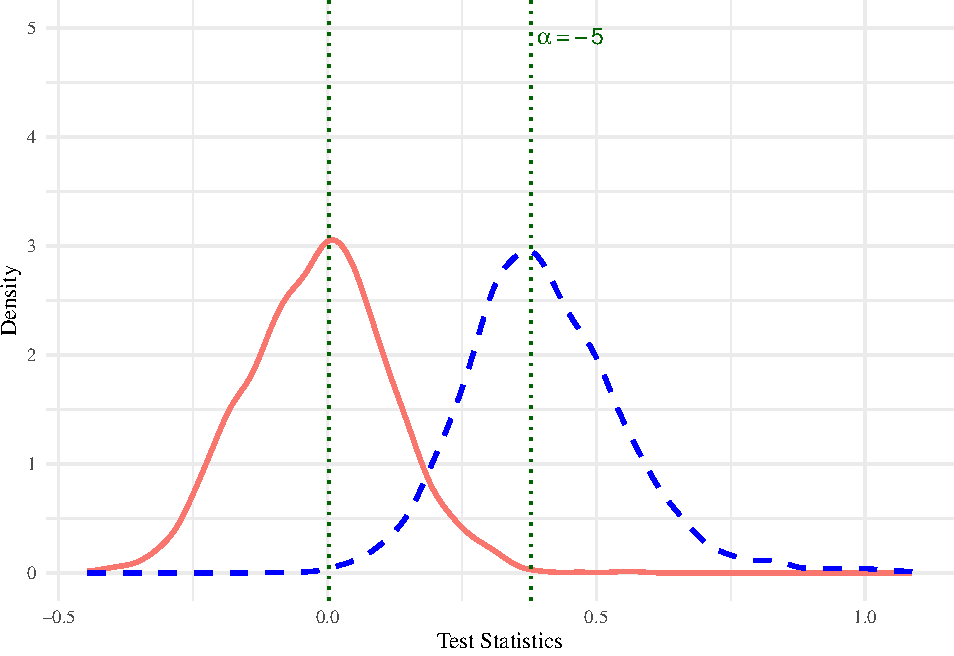
\includegraphics[scale=0.4]{./Figures/Plot_empirical_test-1} \vspace{-0.4cm}

\begin{figure}[H]
  \centering
  \begin{subfigure}[b]{0.3\textwidth}
    \centering
    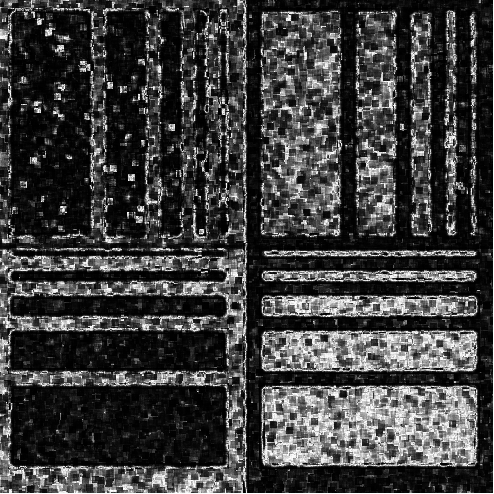
\includegraphics[width=\textwidth]{../../Figures/PNG/H_pvalue_Phantom_4_z1_200b}
    \caption{$S_{\widetilde{H}_{\text{AO}}}(\bm{Z}; L)$}
    \label{fig:sim_SAR_Images-1}
  \end{subfigure}
  \hfill
  \begin{subfigure}[b]{0.3\textwidth}
    \centering
    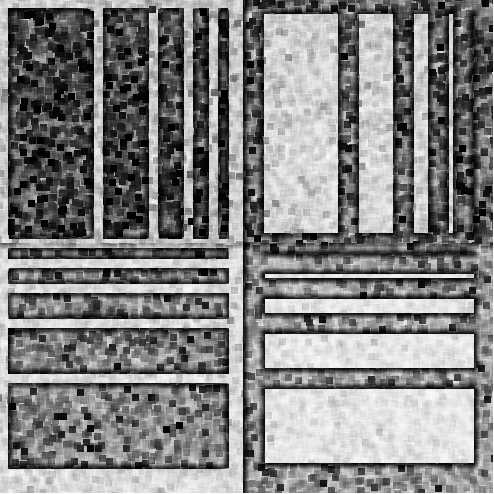
\includegraphics[width=\textwidth]{../../Figures/PNG/cv_pvalues_Phantom_4_z1}
    \caption{$T_\text{CV}$}
    \label{fig:sim_SAR_Images-2}
  \end{subfigure}
  \hfill
  \begin{subfigure}[b]{0.3\textwidth}
    \centering
    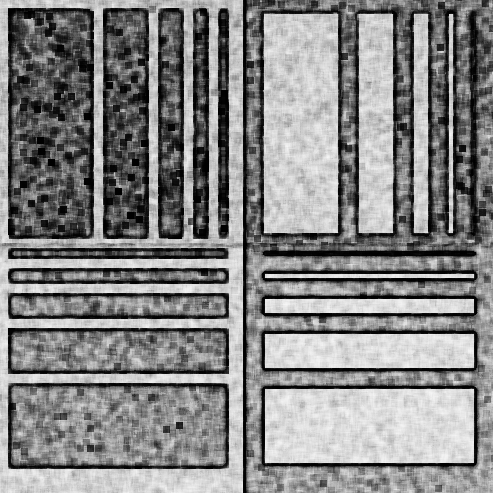
\includegraphics[width=\textwidth]{../../Figures/PNG/mnad_p_values_Phantom_mnad_7_z1}
     \caption{$T_{\text{CV}_{\text{MnAD}}}$}
    \label{fig:sim_SAR_Images-3}
  \end{subfigure}
  \caption{Map of $p$-values of simulated image for each test. }
  \label{fig:sim_SAR_Images}
\end{figure}
 
\end{frame} 



\begin{frame} \frametitle{\large{Simulated Data }}\vspace{-0.1cm}
%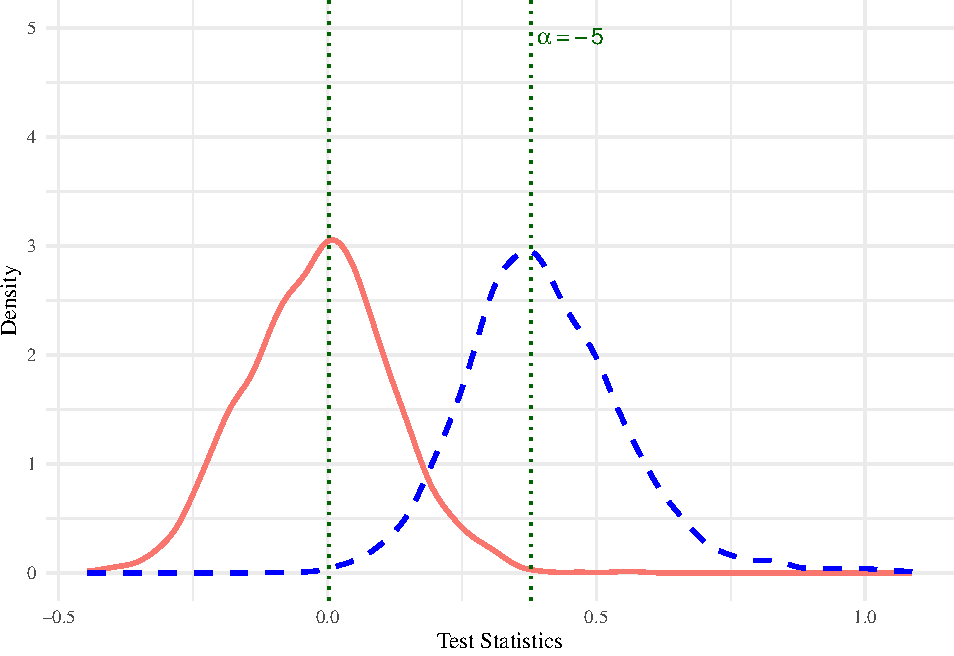
\includegraphics[scale=0.4]{./Figures/Plot_empirical_test-1} \vspace{-0.4cm}

\begin{figure}[H]
  \centering
  \begin{subfigure}[b]{0.3\textwidth}
    \centering
    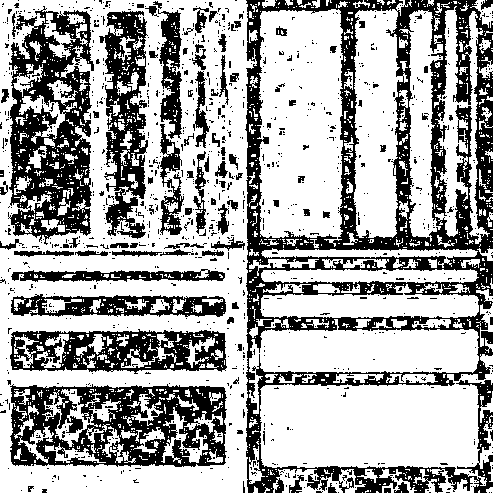
\includegraphics[width=\textwidth]{../../Figures/PNG/H_005_Phantom_4_z1_AO_200b}
    \caption{$S_{\widetilde{H}_{\text{AO}}}(\bm{Z}; L)$}
    \label{fig:sim_SAR_Images_p05-1}
  \end{subfigure}
  \hfill
  \begin{subfigure}[b]{0.3\textwidth}
    \centering
    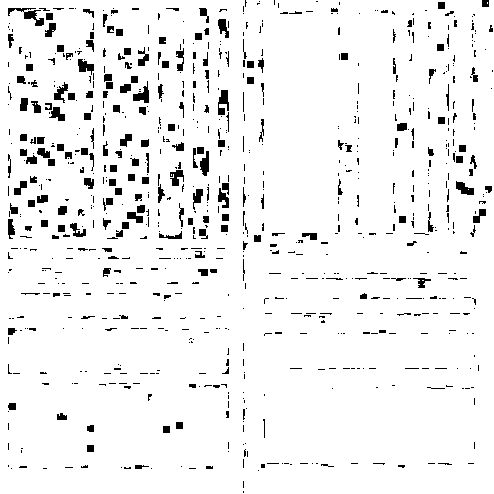
\includegraphics[width=\textwidth]{../../Figures/PNG/cv_005_pvalues_Phantom_4_z1}
    \caption{$T_\text{CV}$}
    \label{fig:sim_SAR_Images_p05-2}
  \end{subfigure}
  \hfill
  \begin{subfigure}[b]{0.3\textwidth}
    \centering
    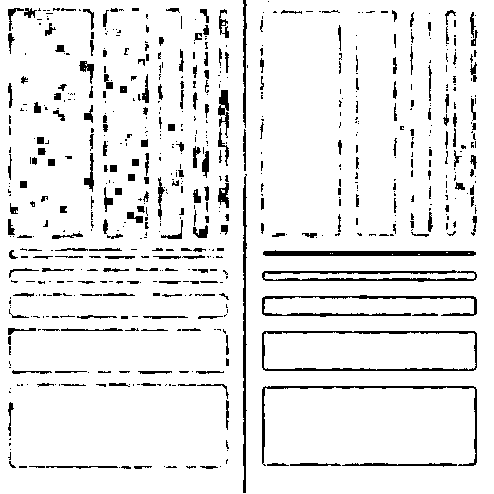
\includegraphics[width=\textwidth]{../../Figures/PNG/mnad_005_Phantom_7_z1}
     \caption{$T_{\text{CV}_{\text{MnAD}}}$}
    \label{fig:sim_SAR_Images_p05-3}
  \end{subfigure}
  \caption{Results for a threshold of $0.05$ of the $p$-value of simulated image for each test. }
  \label{fig:sim_SAR_Images_p05}
\end{figure}
 
\end{frame} 


\begin{frame} \frametitle{\large{SAR Data }}\vspace{-0.1cm}
%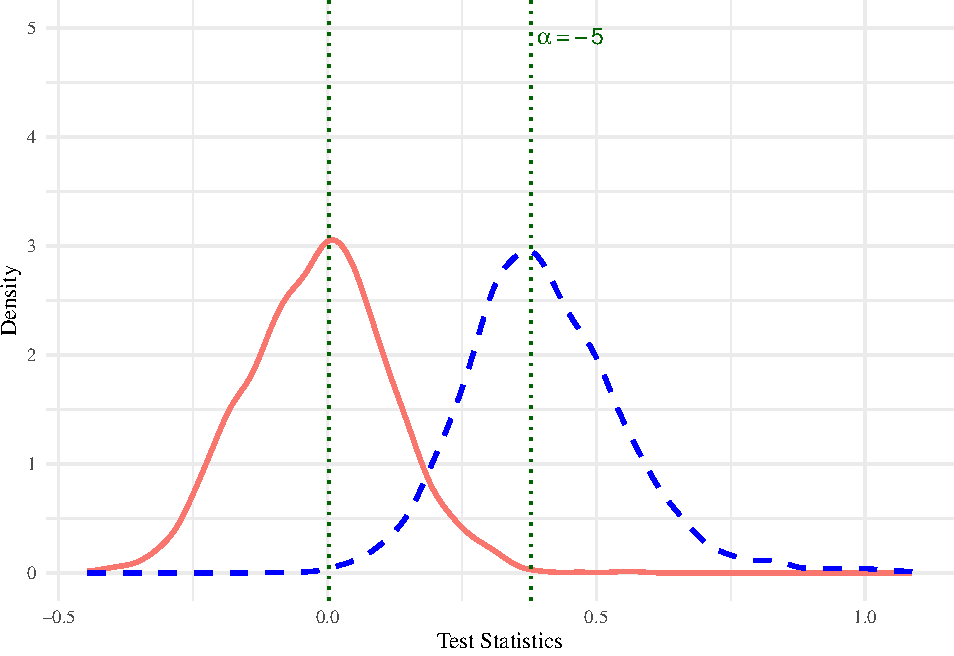
\includegraphics[scale=0.4]{./Figures/Plot_empirical_test-1} \vspace{-0.4cm}

\begin{figure}[H]
  \centering
  \begin{subfigure}[b]{0.3\textwidth}
    \centering
    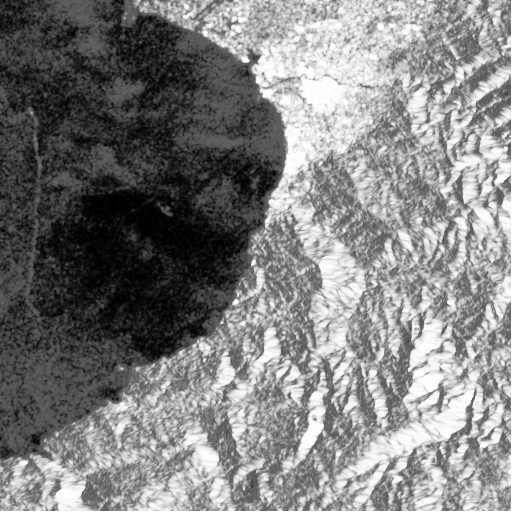
\includegraphics[width=\textwidth]{../../Figures/PNG/Mexico_512}
    \caption{Coast of Jalisco, $L=18$}
    \label{fig:real_SAR_Images_coe-1}
  \end{subfigure}
  \hfill
  \begin{subfigure}[b]{0.3\textwidth}
    \centering
    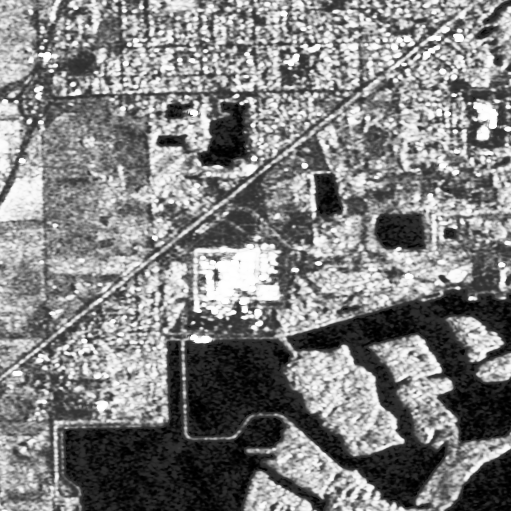
\includegraphics[width=\textwidth]{../../Figures/PNG/lake_512}
    \caption{Illinois-Region 1, $L=36$}
    \label{fig:real_SAR_Images_coe-2}
  \end{subfigure}
  \hfill
  \begin{subfigure}[b]{0.3\textwidth}
    \centering
    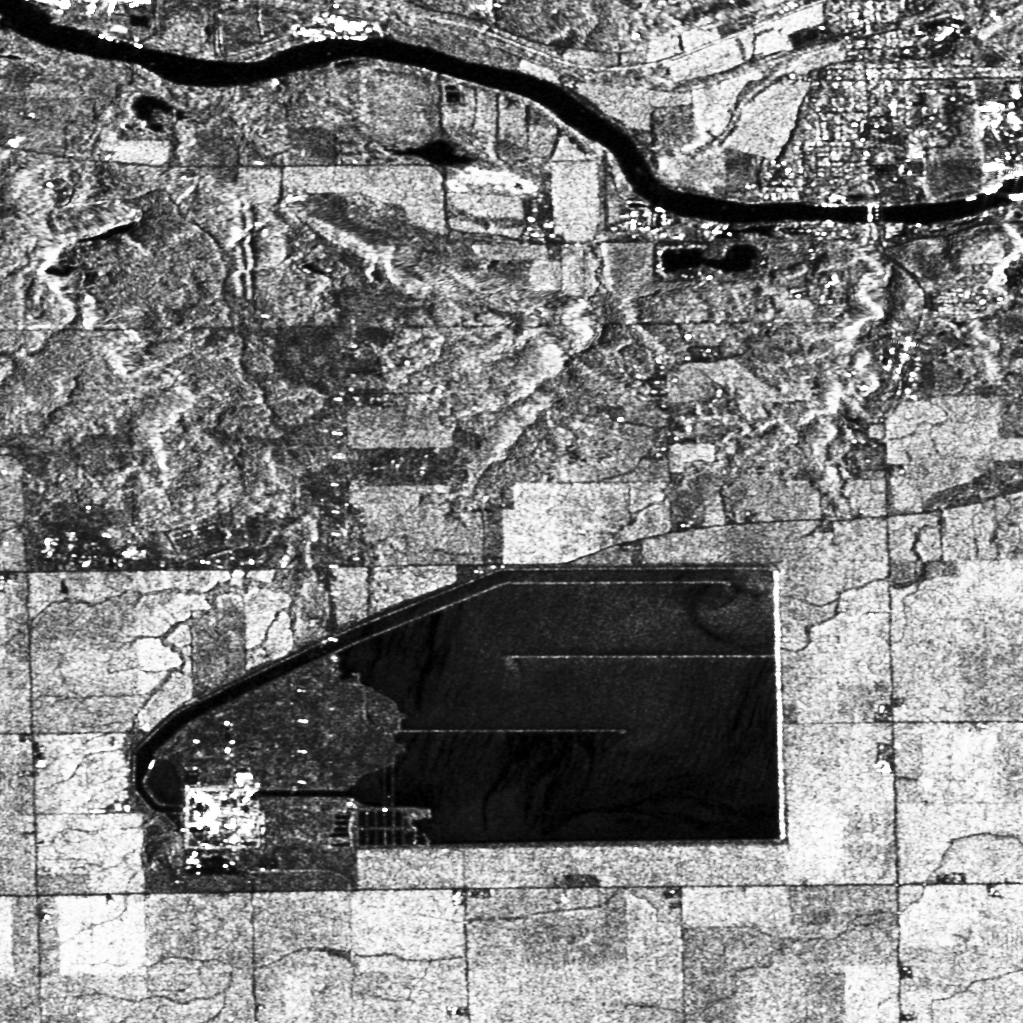
\includegraphics[width=\textwidth]{../../Figures/PNG/Illinois_1024_36L}
     \caption{Illinois-Region 2,  $L=36$}
    \label{fig:real_SAR_Images_coe-3}
  \end{subfigure}
  \caption{SAR images. }
  \label{fig:real_SAR_Images_coe}
\end{figure}
\end{frame} 



\begin{frame} \frametitle{\large{SAR Data, Coast of Jalisco-Mexico }}\vspace{-0.1cm}
%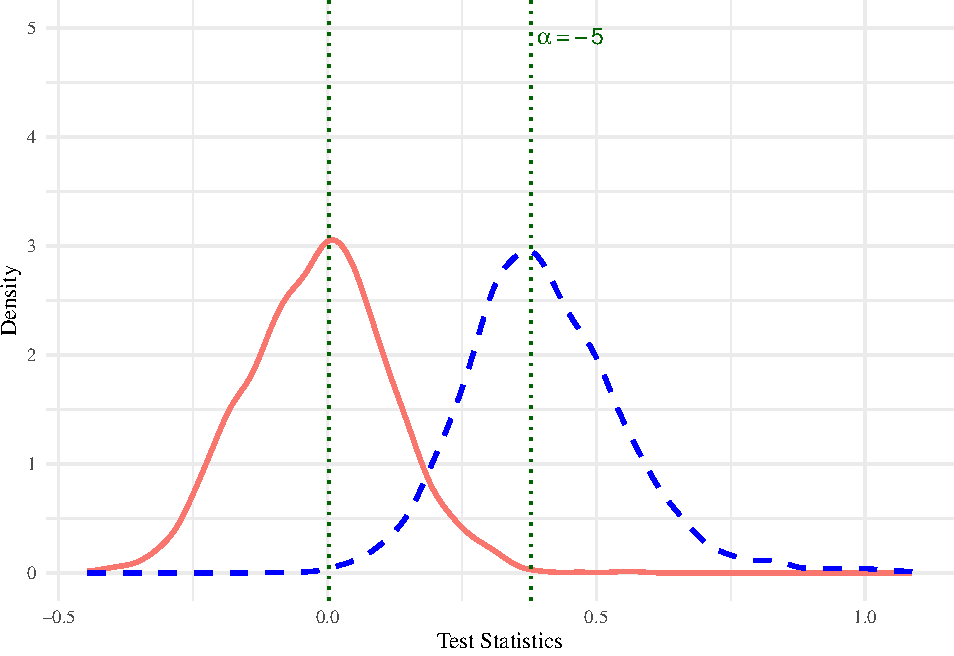
\includegraphics[scale=0.4]{./Figures/Plot_empirical_test-1} \vspace{-0.4cm}

\begin{figure}[H]
  \centering
  \begin{subfigure}[b]{0.3\textwidth}
    \centering
    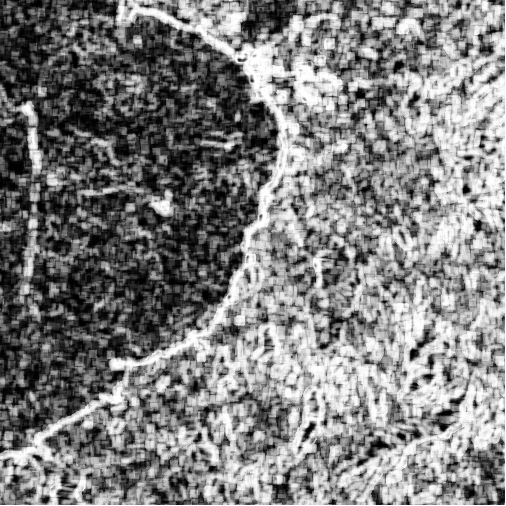
\includegraphics[width=\textwidth]{../../Figures/PNG/Entropy_Mexico_512_18L_AO_200b}
    \caption{$S_{\widetilde{H}_{\text{AO}}}(\bm{Z}; L)$}
    \label{fig:real_images_test_Mexico-1}
  \end{subfigure}
  \hfill
  \begin{subfigure}[b]{0.3\textwidth}
    \centering
    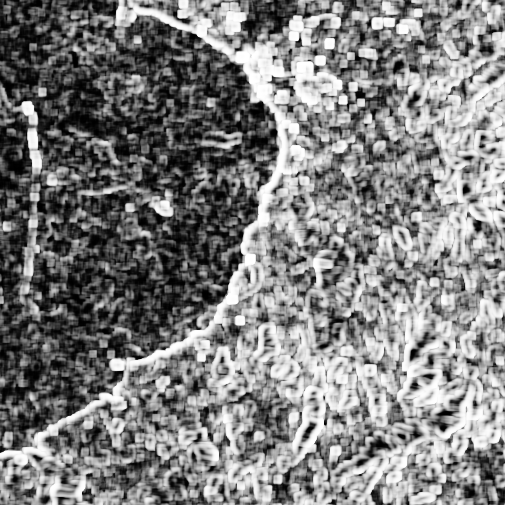
\includegraphics[width=\textwidth]{../../Figures/PNG/cv_mexico_512}
    \caption{$T_\text{CV}$}
    \label{fig:real_images_test_Mexico-2}
  \end{subfigure}
  \hfill
  \begin{subfigure}[b]{0.3\textwidth}
    \centering
    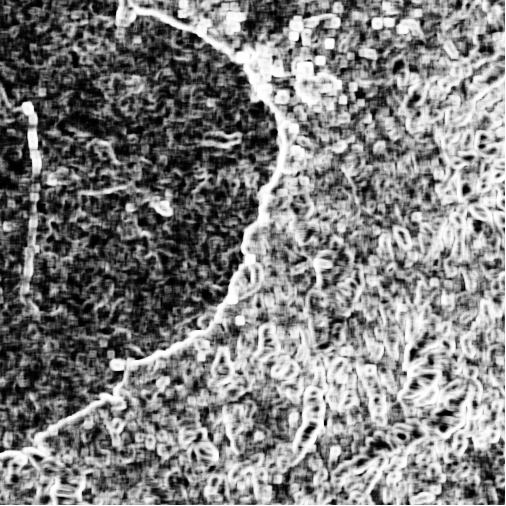
\includegraphics[width=\textwidth]{../../Figures/PNG/mnad_mexico_512}
    \caption{$T_{\text{CV}_{\text{MnAD}}}$}
    \label{fig:real_images_test_Mexico-3}
  \end{subfigure}
  \caption{Results of applying the test statistics.}
  \label{fig:real_images_test_Mexico}
\end{figure}

\end{frame} 

\begin{frame} \frametitle{\large{SAR Data, Coast of Jalisco-Mexico }}\vspace{-0.1cm}
%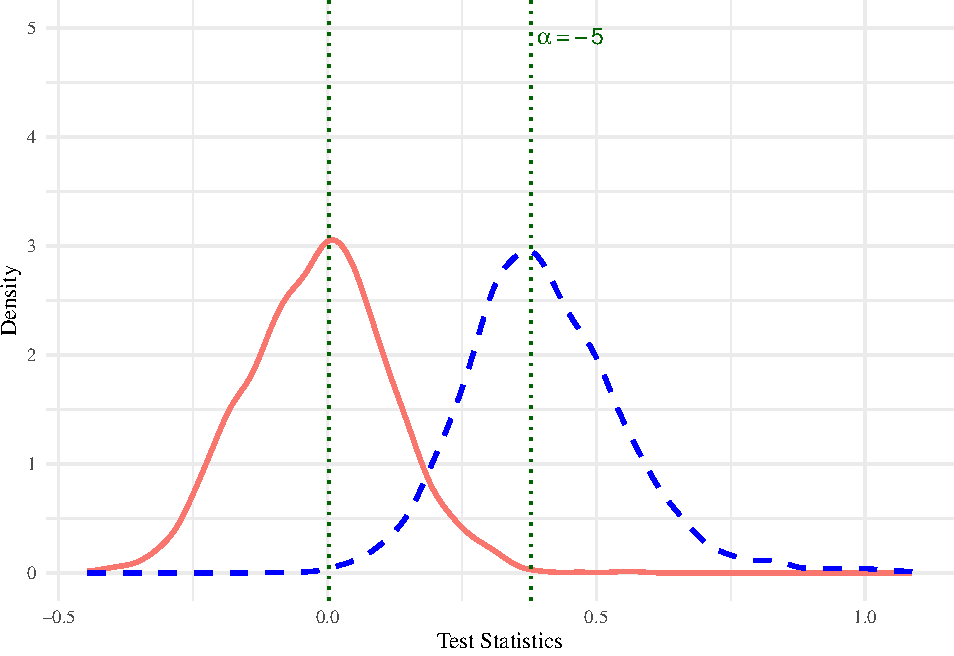
\includegraphics[scale=0.4]{./Figures/Plot_empirical_test-1} \vspace{-0.4cm}

\begin{figure}[H]
  \centering
  \begin{subfigure}[b]{0.3\textwidth}
    \centering
    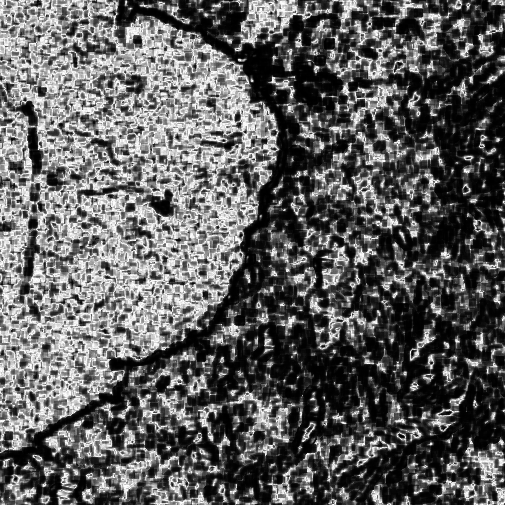
\includegraphics[width=\textwidth]{../../Figures/PNG/H_pvalue_Mexico_512_18L_AO_200b}
    \caption{$S_{\widetilde{H}_{\text{AO}}}(\bm{Z}; L)$}
    \label{fig:Mexico_pvalue-1}
  \end{subfigure}
  \hfill
  \begin{subfigure}[b]{0.3\textwidth}
    \centering
    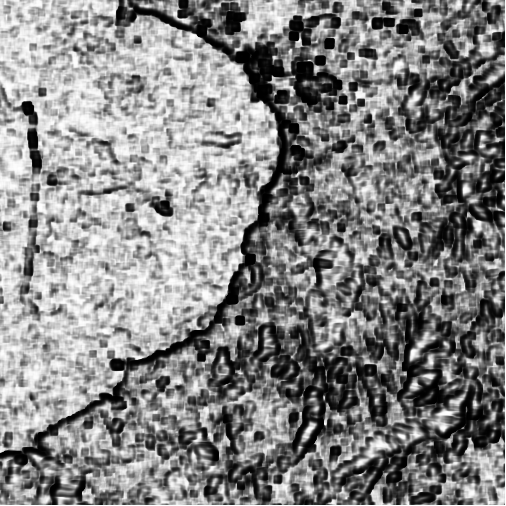
\includegraphics[width=\textwidth]{../../Figures/PNG/cv_pvalues_mexico_512}
    \caption{$T_\text{CV}$}
    \label{fig:Mexico_pvalue-2}
  \end{subfigure}
  \hfill
  \begin{subfigure}[b]{0.3\textwidth}
    \centering
    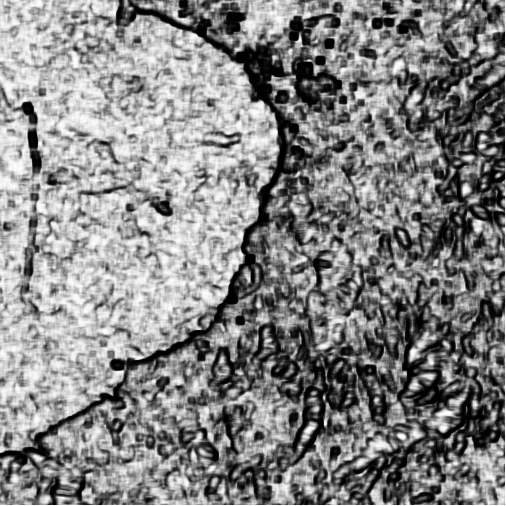
\includegraphics[width=\textwidth]{../../Figures/PNG/mnad_p_values_mexico_512}
     \caption{$T_{\text{CV}_{\text{MnAD}}}$}
    \label{fig:Mexico_pvalue-3}
  \end{subfigure}
  \caption{Map of $p$-values of Coast of Jalisco image for each test. }
  \label{fig:Mexico_pvalue}
\end{figure}
\end{frame} 


\begin{frame} \frametitle{\large{SAR Data, Coast of Jalisco-Mexico }}\vspace{-0.1cm}
%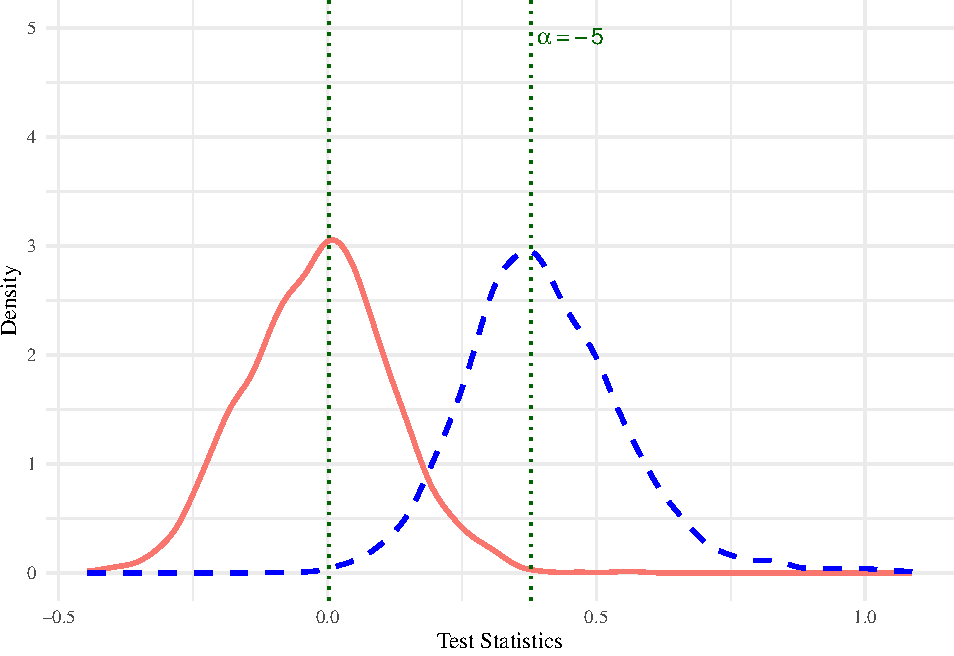
\includegraphics[scale=0.4]{./Figures/Plot_empirical_test-1} \vspace{-0.4cm}
\begin{figure}[H]
  \centering
  \begin{subfigure}[b]{0.3\textwidth}
    \centering
    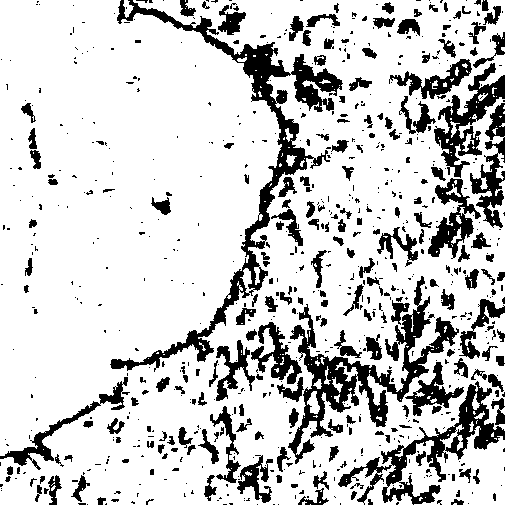
\includegraphics[width=\textwidth]{../../Figures/PNG/H_005__Mexico_512_18L_AO_200b}
    \caption{$S_{\widetilde{H}_{\text{AO}}}(\bm{Z}; L)$}
    \label{fig:Mexico_crops_0.05-1}
  \end{subfigure}
  \hfill
  \begin{subfigure}[b]{0.3\textwidth}
    \centering
    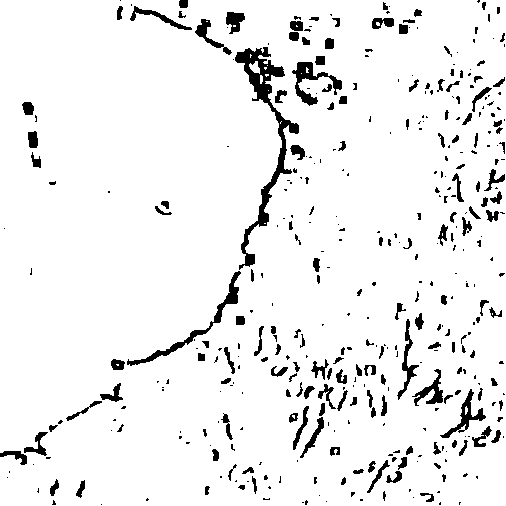
\includegraphics[width=\textwidth]{../../Figures/PNG/cv_005_pvalues_mexico_512}
    \caption{$T_\text{CV}$}
    \label{fig:Mexico_crops_0.05-2}
  \end{subfigure}
  \hfill
  \begin{subfigure}[b]{0.3\textwidth}
    \centering
    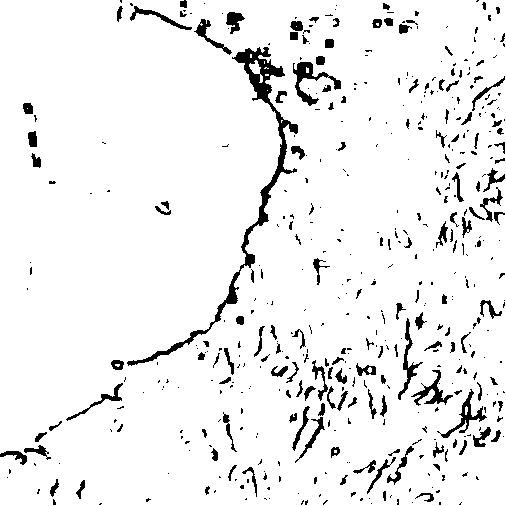
\includegraphics[width=\textwidth]{../../Figures/PNG/mnad_005_mexico_512}
     \caption{$T_{\text{CV}_{\text{MnAD}}}$}
    \label{fig:Mexico_crops_0.05-3}
  \end{subfigure}
  \caption{Results for a threshold of $0.05$ of the $p$-value of Coast of Jalisco for each test. }
  \label{fig:Mexico_crops_0.05}
\end{figure}
\end{frame} 



\begin{frame} \frametitle{\large{SAR Data, Illinois-Region 1 }}\vspace{-0.1cm}
%\includegraphics[scale=0.4]{./Figures/Plot_empirical_test-1} \vspace{-0.4cm}
\begin{figure}[H]
  \centering
  \begin{subfigure}[b]{0.3\textwidth}
    \centering
    \includegraphics[width=\textwidth]{../../Figures/PNG/Entropy_lake_512_36L_AO_100b}
    \caption{$S_{\widetilde{H}_{\text{AO}}}(\bm{Z}; L)$}
    \label{fig:test_lake-1}
  \end{subfigure}
  \hfill
  \begin{subfigure}[b]{0.3\textwidth}
    \centering
    \includegraphics[width=\textwidth]{../../Figures/PNG/cv_lake_512}
    \caption{$T_\text{CV}$}
    \label{fig:test_lake-2}
  \end{subfigure}
  \hfill
  \begin{subfigure}[b]{0.3\textwidth}
    \centering
    \includegraphics[width=\textwidth]{../../Figures/PNG/mnad_lake_512}
    \caption{$T_{\text{CV}_{\text{MnAD}}}$}
    \label{fig:test_lake-3}
  \end{subfigure}
  \caption{Results of applying the test statistics, Illinois-Region 1.}
  \label{fig:test_lake}
\end{figure}
\end{frame} 


\begin{frame} \frametitle{\large{SAR Data, Illinois-Region 1 }}\vspace{-0.1cm}
%\includegraphics[scale=0.4]{./Figures/Plot_empirical_test-1} \vspace{-0.4cm}
\begin{figure}[H]
  \centering
  \begin{subfigure}[b]{0.3\textwidth}
    \centering
    \includegraphics[width=\textwidth]{../../Figures/PNG/H_pvalue_lake_512_36L_AO_100b}
    \caption{$S_{\widetilde{H}_{\text{AO}}}(\bm{Z}; L)$}
    \label{fig:lake_pvalue-1}
  \end{subfigure}
  \hfill
  \begin{subfigure}[b]{0.3\textwidth}
    \centering
    \includegraphics[width=\textwidth]{../../Figures/PNG/cv_pvalues_lake_512}
    \caption{$T_\text{CV}$}
    \label{fig:lake_pvalue-2}
  \end{subfigure}
  \hfill
  \begin{subfigure}[b]{0.3\textwidth}
    \centering
    \includegraphics[width=\textwidth]{../../Figures/PNG/mnad_p_values_lake_512}
     \caption{$T_{\text{CV}_{\text{MnAD}}}$}
    \label{fig:lake_pvalue-3}
  \end{subfigure}
  \caption{Map of $p$-values, Illinois-Region 1. }
  \label{fig:lake_pvalue}
\end{figure}
\end{frame} 


\begin{frame} \frametitle{\large{SAR Data, Illinois-Region 1 }}\vspace{-0.1cm}
%\includegraphics[scale=0.4]{./Figures/Plot_empirical_test-1} \vspace{-0.4cm}
\begin{figure}[H]
  \centering
  \begin{subfigure}[b]{0.3\textwidth}
    \centering
    \includegraphics[width=\textwidth]{../../Figures/PNG/H_005_lake_512_36L_AO_100b}
    \caption{$S_{\widetilde{H}_{\text{AO}}}(\bm{Z}; L)$}
    \label{fig:lake_0.05-1}
  \end{subfigure}
  \hfill
  \begin{subfigure}[b]{0.3\textwidth}
    \centering
    \includegraphics[width=\textwidth]{../../Figures/PNG/cv_005_pvalues_lake_512}
    \caption{$T_\text{CV}$}
    \label{fig:lake_0.05-2}
  \end{subfigure}
  \hfill
  \begin{subfigure}[b]{0.3\textwidth}
    \centering
    \includegraphics[width=\textwidth]{../../Figures/PNG/mnad_005_lake_512}
     \caption{$T_{\text{CV}_{\text{MnAD}}}$}
    \label{fig:lake_0.05-3}
  \end{subfigure}
  \caption{Results for a threshold of $0.05$ of the $p$-value, Illinois-Region 1. }
  \label{fig:lake_0.05}
\end{figure}
\end{frame} 

\begin{frame} \frametitle{\large{SAR Data, Illinois-Region 1 }}\vspace{-0.1cm}
%\includegraphics[scale=0.4]{./Figures/Plot_empirical_test-1} \vspace{-0.4cm}
\begin{figure}[H]
  \centering
  \begin{subfigure}[b]{0.3\textwidth}
    \centering
    \includegraphics[width=\textwidth]{../../Figures/PNG/H_005_lake_512_36L_AO_100b}
    \caption{$S_{\widetilde{H}_{\text{AO}}}(\bm{Z}; L)$}
    \label{fig:lake_0.05-1}
  \end{subfigure}
  \hfill
  \begin{subfigure}[b]{0.3\textwidth}
    \centering
    \includegraphics[width=\textwidth]{../../Figures/PNG/cv_005_pvalues_lake_512}
    \caption{$T_\text{CV}$}
    \label{fig:lake_0.05-2}
  \end{subfigure}
  \hfill
  \begin{subfigure}[b]{0.3\textwidth}
    \centering
    \includegraphics[width=\textwidth]{../../Figures/PNG/mnad_005_lake_512}
     \caption{$T_{\text{CV}_{\text{MnAD}}}$}
    \label{fig:lake_0.05-3}
  \end{subfigure}
  \caption{Results for a threshold of $0.05$ of the $p$-value, Illinois-Region 1. }
  \label{fig:lake_0.05}
\end{figure}
\end{frame} 


\begin{frame} \frametitle{\large{SAR Data, Illinois-Region 2 }}\vspace{-0.1cm}
\begin{figure}[H]
  \centering
  \begin{subfigure}[b]{0.3\textwidth}
    \centering
    \includegraphics[width=\textwidth]{../../Figures/PNG/Entropy_Illinois_1024_36L_AO_200b}
    \caption{$S_{\widetilde{H}_{\text{AO}}}(\bm{Z}; L)$}
    \label{fig:real_images_test_Illinois-1}
  \end{subfigure}
  \hfill
  \begin{subfigure}[b]{0.3\textwidth}
    \centering
    \includegraphics[width=\textwidth]{../../Figures/PNG/cv_Illinois_crops_1024}
    \caption{$T_\text{CV}$}
    \label{fig:real_images_test_Illinois-2}
  \end{subfigure}
  \hfill
  \begin{subfigure}[b]{0.3\textwidth}
    \centering
    \includegraphics[width=\textwidth]{../../Figures/PNG/mnad_Illinois_crops_1024}
    \caption{$T_{\text{CV}_{\text{MnAD}}}$}
    \label{fig:real_images_test_Illinois-3}
  \end{subfigure}
  \caption{Results of applying the test statistics, Illinois-Region 2.}
  \label{fig:real_images_test_Illinois}
\end{figure}
\end{frame} 


\begin{frame} \frametitle{\large{SAR Data, Illinois-Region 2 }}\vspace{-0.1cm}
\begin{figure}[H]
  \centering
  \begin{subfigure}[b]{0.3\textwidth}
    \centering
    \includegraphics[width=\textwidth]{../../Figures/PNG/H_pvalue_Illinois_1024_36L_AO_200b}
    \caption{$S_{\widetilde{H}_{\text{AO}}}(\bm{Z}; L)$}
    \label{fig:Illinois_crops_pvalue-1}
  \end{subfigure}
  \hfill
  \begin{subfigure}[b]{0.3\textwidth}
    \centering
    \includegraphics[width=\textwidth]{../../Figures/PNG/cv_pvalues_Illinois_crops_1024}
    \caption{$T_\text{CV}$}
    \label{fig:Illinois_crops_pvalue-2}
  \end{subfigure}
  \hfill
  \begin{subfigure}[b]{0.3\textwidth}
    \centering
    \includegraphics[width=\textwidth]{../../Figures/PNG/mnad_p_values_Illinois_crops_1024}
     \caption{$T_{\text{CV}_{\text{MnAD}}}$}
    \label{fig:Illinois_crops_pvalue-3}
  \end{subfigure}
  \caption{Map of $p$-values, Illinois-Region 2. }
  \label{fig:Illinois_crops_pvalue}
\end{figure}
\end{frame} 

\begin{frame} \frametitle{\large{SAR Data, Illinois-Region 2 }}\vspace{-0.1cm}
\begin{figure}[H]
  \centering
  \begin{subfigure}[b]{0.3\textwidth}
    \centering
    \includegraphics[width=\textwidth]{../../Figures/PNG/H_005_pvalues_Illinois_1024_36L_AO_200b}
    \caption{$S_{\widetilde{H}_{\text{AO}}}(\bm{Z}; L)$}
    \label{fig:Illinois_crops_0.05-1}
  \end{subfigure}
  \hfill
  \begin{subfigure}[b]{0.3\textwidth}
    \centering
    \includegraphics[width=\textwidth]{../../Figures/PNG/cv_005_pvalues_Illinois_crops_1024}
    \caption{$T_\text{CV}$}
    \label{fig:Illinois_crops_0.05-2}
  \end{subfigure}
  \hfill
  \begin{subfigure}[b]{0.3\textwidth}
    \centering
    \includegraphics[width=\textwidth]{../../Figures/PNG/mnad_005_Illinois_crops_1024}
     \caption{$T_{\text{CV}_{\text{MnAD}}}$}
    \label{fig:Illinois_crops_0.05-3}
  \end{subfigure}
  \caption{Results for a threshold of $0.05$ of the $p$-value, Illinois-Region 2. }
  \label{fig:Illinois_crops_0.05}
\end{figure}
\end{frame} 




%----------------------------------------------------

\section{Conclusions \& Future Perspectives}
\begin{frame} 
    \frametitle{\large{Conclusions \& Future Perspectives}}
    \vspace{-0.5cm}

    \justifying
    \begin{columns}[T,onlytextwidth]
        \begin{column}{.99\textwidth}
            \begin{exampleblock}{}\justifying
			This work provides a practical and theoretical answer to the
following physical question: How to detect heterogeneity in SAR images,
assuming that the SAR intensity follows the \(\Gamma_{\text{SAR}}\)
model.   
                \begin{itemize}
                    \item We proposed three novel hypothesis tests, one from
the Shannon entropy and two from the variation coefficient variants.
                    
                    \item An
application to three recent SAR images was performed. The results showed
that the Shannon entropy-based test was more robust than the CV-based
tests. In addition, all tests could recognize images with different
textures and identify edges where the texture type changes.
                \end{itemize}
								\pause
                We plan to explore the estimation of ENL in polarimetric SAR (PolSAR) data. This extension will involve:
\begin{itemize}
	\item Estimating the test on each of the three intensity channels of fully PolSAR data
	\item Analyzing the joint distribution
	\item Proposing techniques that generalize the test statistic  into the analysis of PolSAR data. 
	
\end{itemize}
                %Currently, we are working on detecting texturelessness in SAR images. To this end, we propose novel hypothesis tests based on classical and variants of the coefficient of variation.
            \end{exampleblock}
        \end{column}
    \end{columns}
    
    \vspace{0.2cm}
\end{frame}



%---------------------------------------------------

%\begin{frame}[standout]
%  Questions?
%\end{frame}
%
%\appendix
%
%
%\begin{frame}[allowframebreaks]{Referências}
%\tiny{Algumas referências \cite{paula2021generalized,paula2017new,jammalamadaka2001topics,cordeiro2014marshall,nadarajah2012general, paula2018extended}}
%\small
%
  %\bibliography{demo}
 %\bibliographystyle{abbrv}
%
%\end{frame}
\begin{frame}
    \frametitle{\large{}}
    \vspace{-0.5cm}
    \centering \large
    \emph{Thank you for your attention}
    
    %\begin{columns}[T,onlytextwidth]
        %\begin{column}{.99\textwidth}
            %\begin{block}{\textbf{Contact}}
                %Alejandro C. Frery\\
                %alejandro.frery@vuw.ac.nz \\
                %\vspace{0.4cm}
                %\emph{Scan to connect}
								%\vspace{0.2cm}
    %\begin{picture}(0,0)
        %\put(-80,-10){\makebox(0,0)[lt]{\includegraphics[width=2.0cm]{./Figures/QRCode-WebPageVUW}}}
    %\end{picture}
%
         %\end{block}
        %\end{column}
    %\end{columns}
    
    
\end{frame}

\end{document}
